


\begin{comment}
%%%
%%%  FIGURE 
%%%
\begin{figure}[h]
\begin{center}
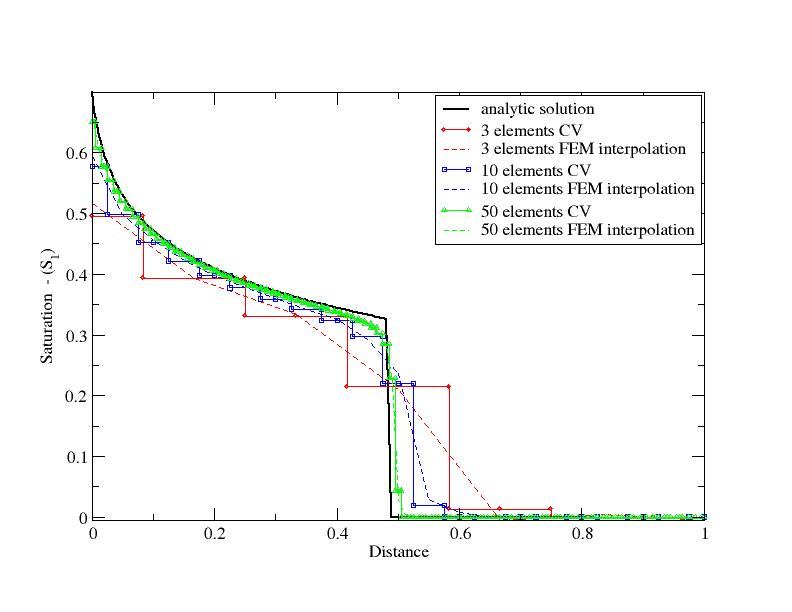
\includegraphics[width=1.\textwidth]{bl-exact-meth-upwind}
\end{center}
\caption{Buckley-Leverett test-cases: Saturation solutions for the continuous upwind method for different 1D P$_{1}$DG-P$_{2}$ mesh resolutions and comparison against standard analytical solution.
\label{bl-exact-meth-upwind}}
\end{figure}

\end{comment}
%%%
%%%  FIGURE 
%%%
\begin{figure}[h]
\vbox{\hbox{\hspace{2.5cm}
    \includegraphics[width=0.62\textwidth]{BL_1d_P0DGP1_convergence.eps}}
\vspace{-.0cm}\hbox{\hspace{2.5cm}
    \includegraphics[width=0.62\textwidth]{BL_1d_P1DGP2_convergence.eps}}
\vspace{-.0cm}\hbox{\hspace{2.5cm}
    \includegraphics[width=0.62\textwidth]{BL_1d_P2DGP3_convergence.eps}}}
    \caption{Buckley-Leverett test-cases: 1-D Saturation profiles for a number of element pairs and grid resolutions -- \PN[0]{1} (top), \PN[1]{2}, \PN[2]{3} (bottom).\label{fig:BL_profiles}}
\end{figure}

%%%
%%%  FIGURE 
%%%
\begin{figure}[h]
\vbox{\hbox{\hspace{1.cm}
    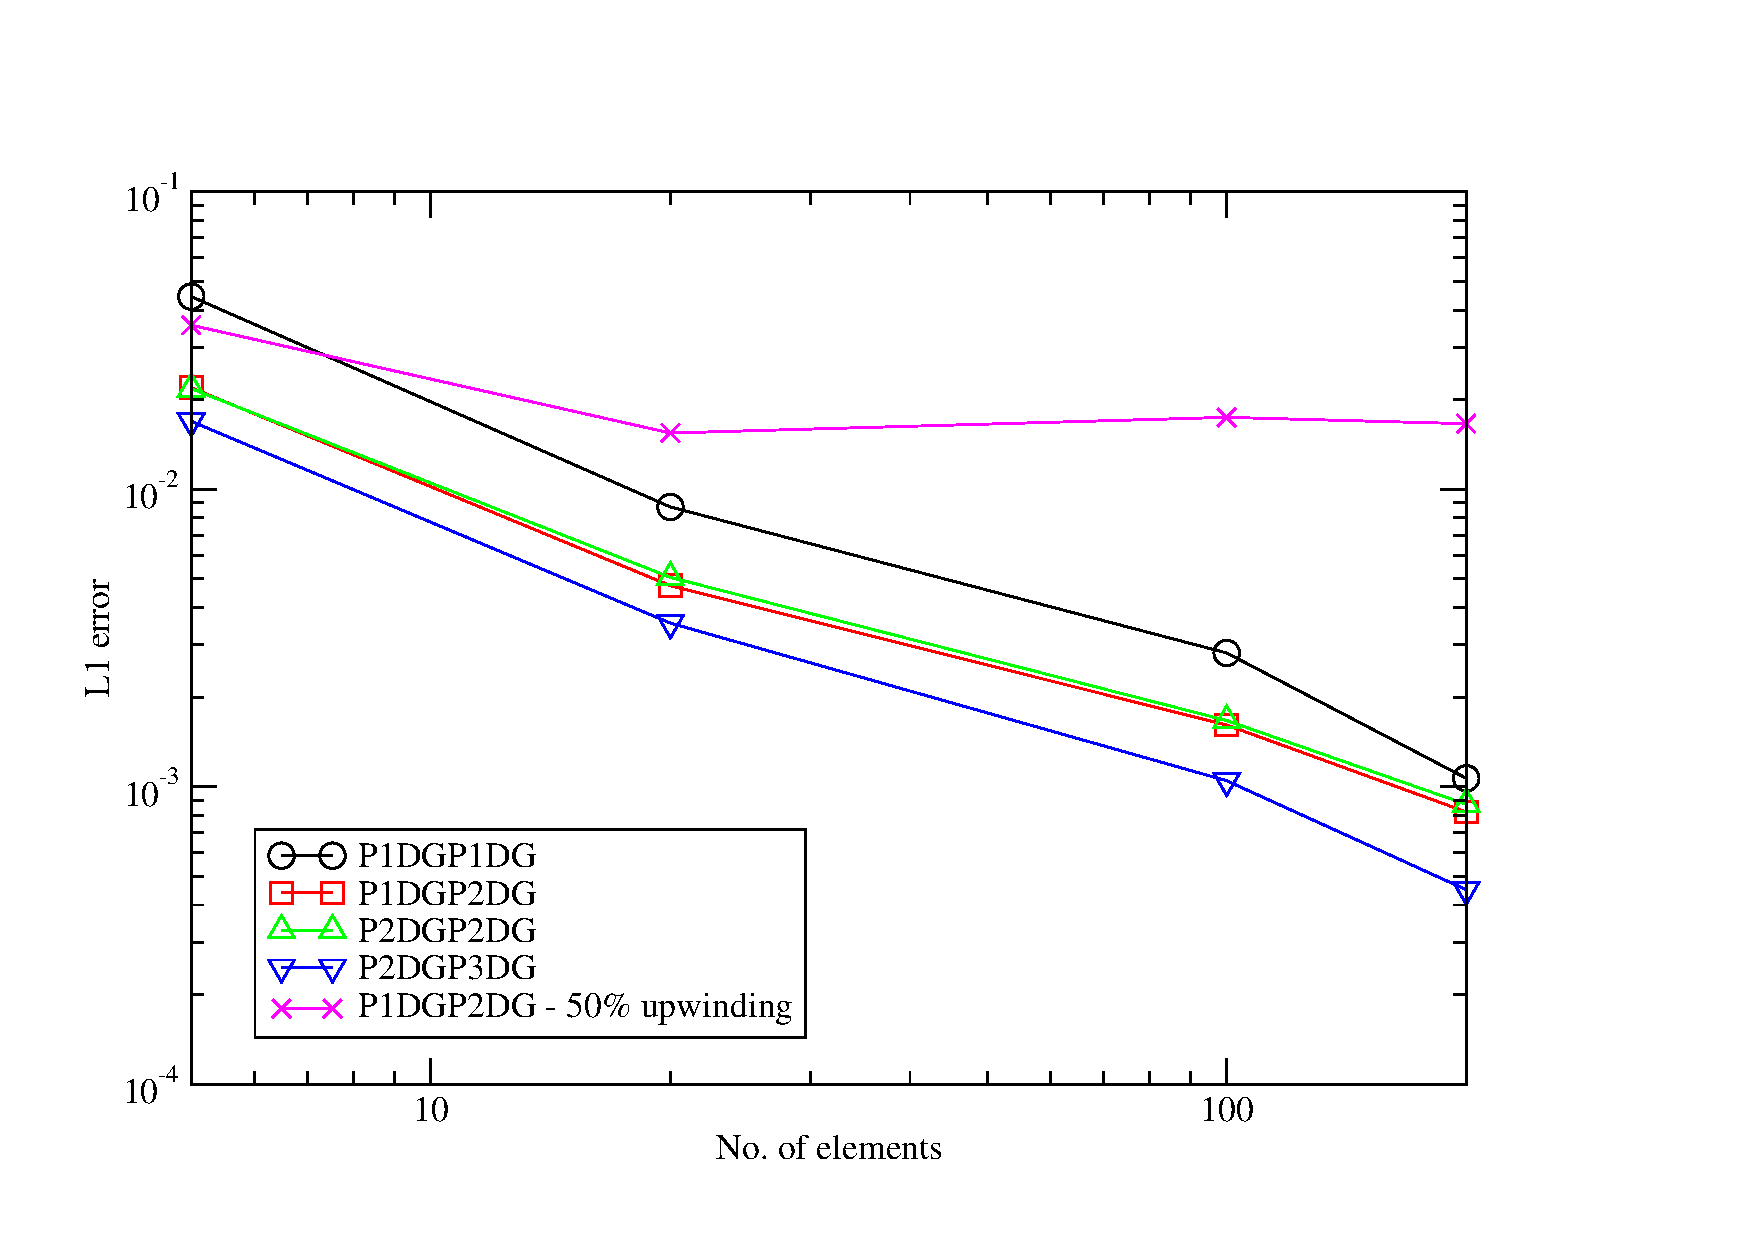
\includegraphics[width=0.8\textwidth]{L1_convergence_rate}}
\vspace{.0cm}\hbox{\hspace{1.cm}
    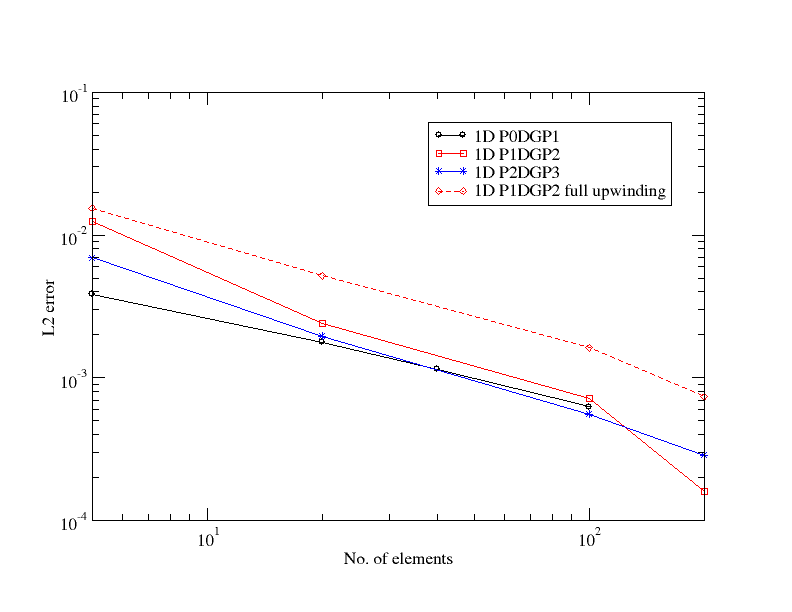
\includegraphics[width=0.8\textwidth]{L2_convergence_rate}}}
    \caption{Buckley-Leverett test-cases: L1 (top) and L2 (bottom) error convergence rates for a number of (continuous) element pairs. \label{fig:BL_converg-rates}}
\end{figure}



%%%
%%%  FIGURE 
%%%
\begin{figure}[h]
\begin{center}
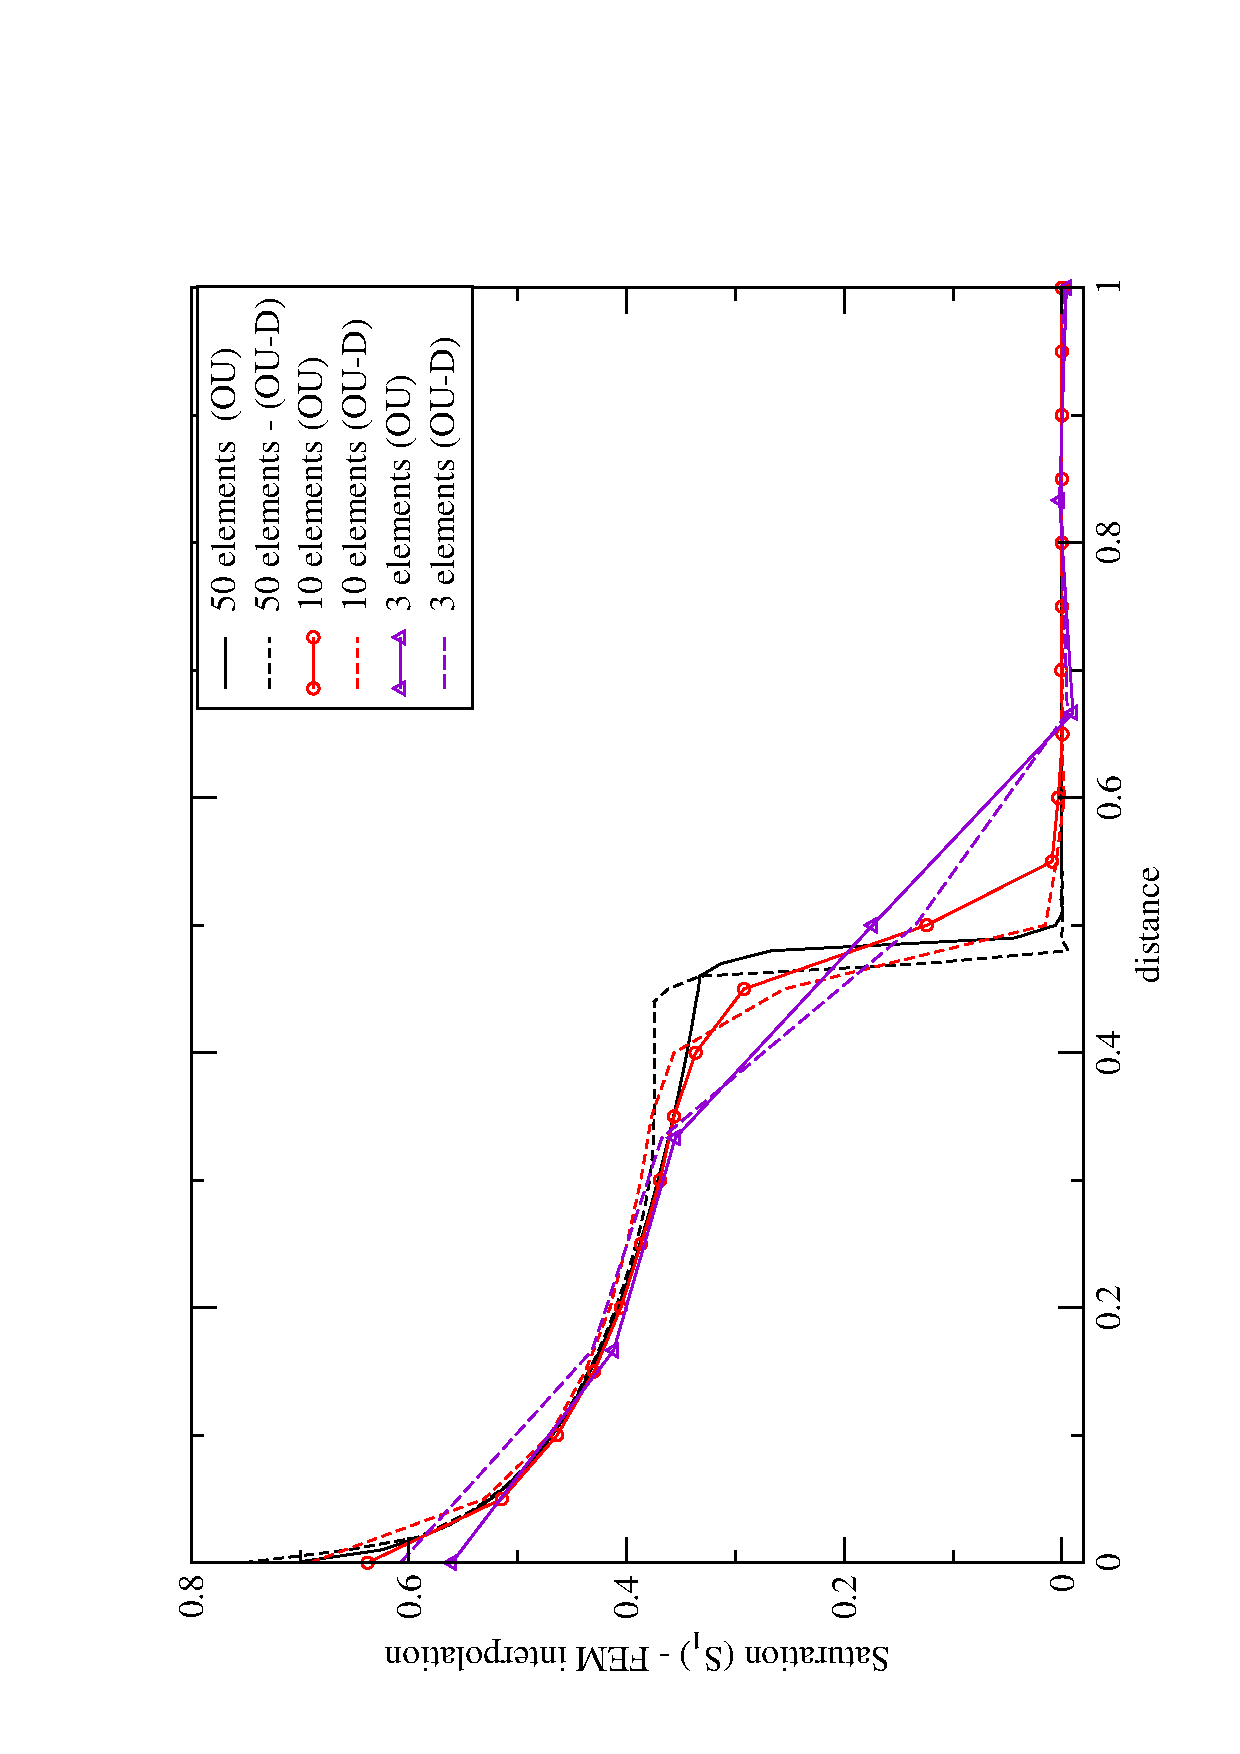
\includegraphics[width=1.\textwidth]{bl-upwind-v-up-and-down}
\end{center}
\caption{Buckley-Leverett test-cases: Comparison of the optimal upwind formulation when using upwinding (OU) and coupled upwind/downwind (OU-D). The finite element interpolation of the saturation field $\left(S_{1}\right)$ is shown at different mesh resolutions. Downwind seems to detract from the accuracy of the solution. \label{bl-upwind-v-up-and-down}}
\end{figure}



\begin{comment}
%%%
%%%  FIGURE 
%%%
\begin{figure}[h]
\vbox{
\begin{center}
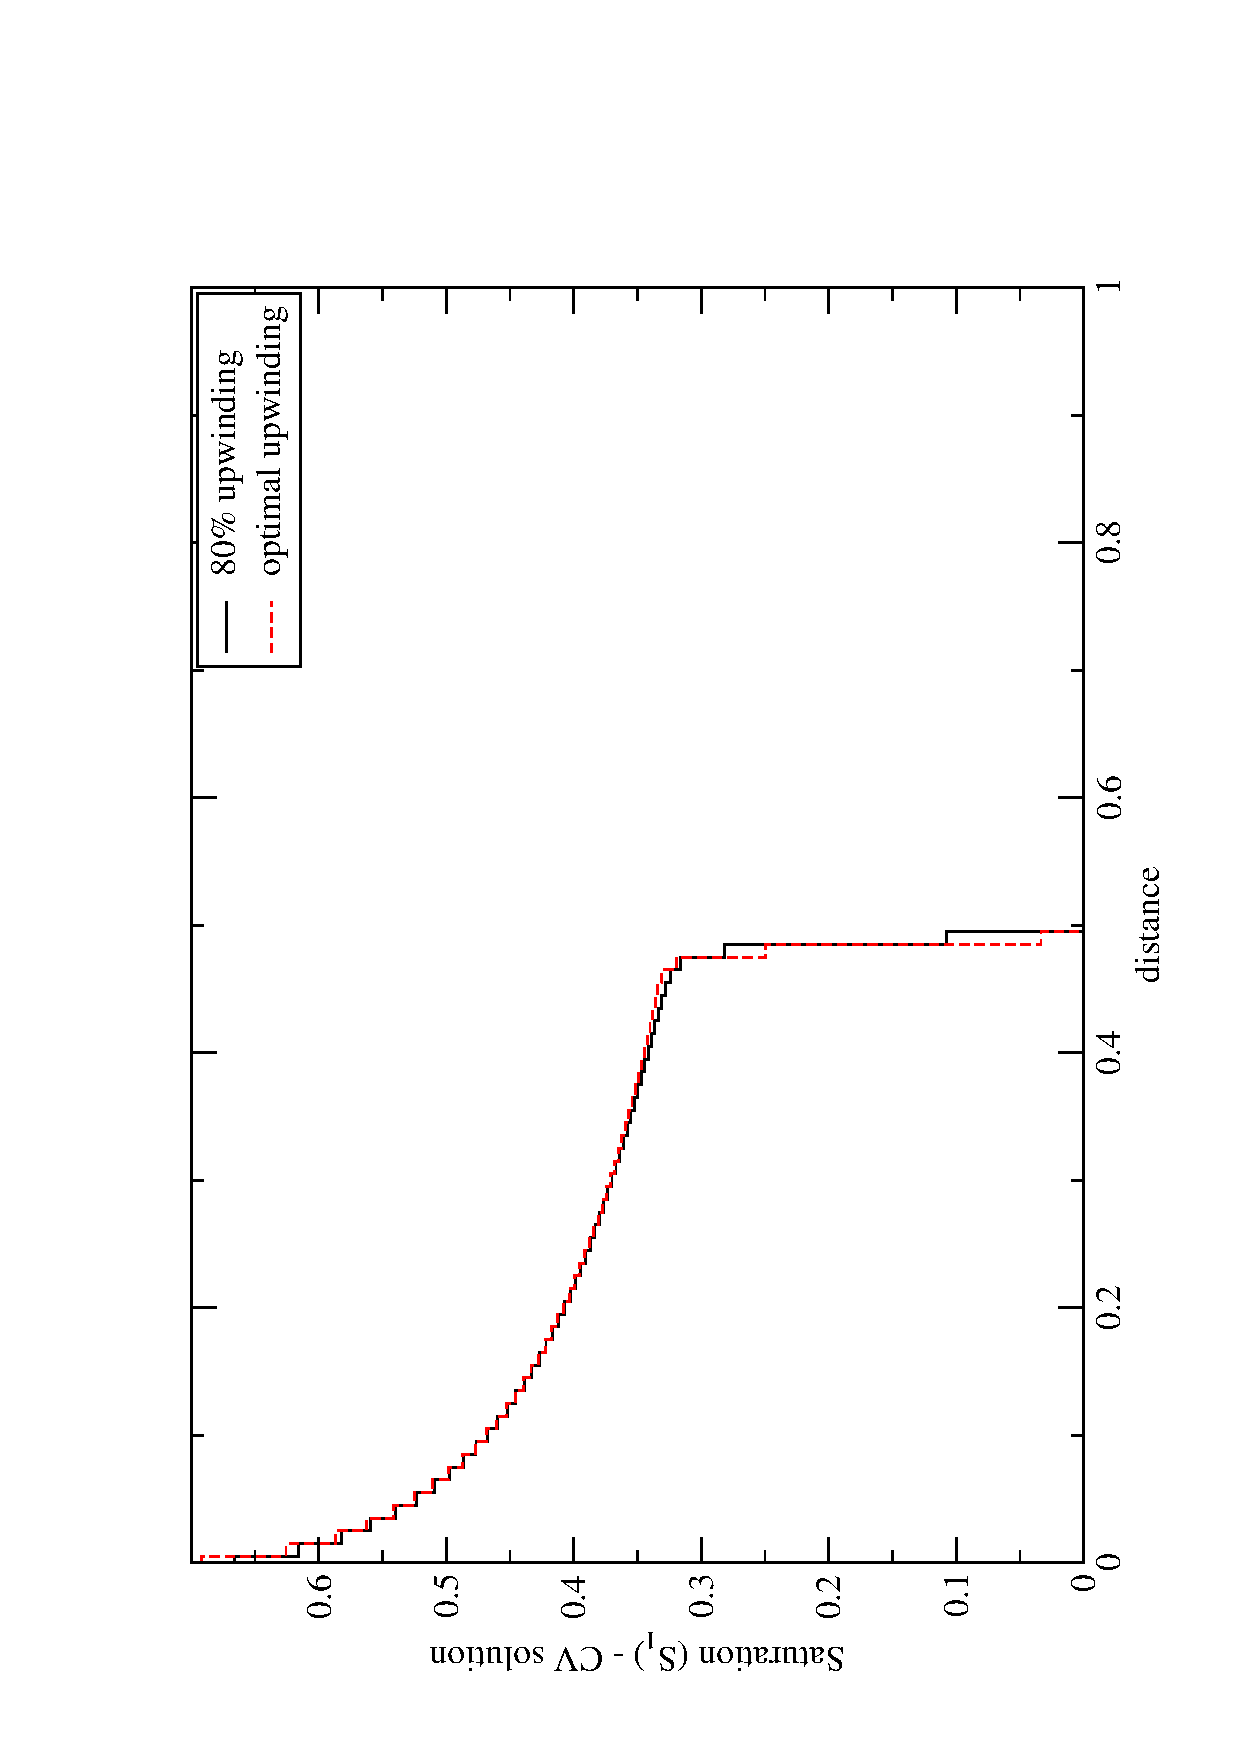
\includegraphics[width=1.\textwidth]{bl-exact-meth-cv-0-8-ele50}
\end{center}
\vspace{0.cm}}
\caption{Buckley-Leverett test-cases: Comparison of control volume solutions using 80$\%$ upwinding and with optimal upwinding and using 50 continuous P$_{1}$DG-P$_{2}$ elements. \label{bl-exact-meth-cv-0-8-ele50}}
\end{figure}

\end{comment}



%%%
%%%  FIGURE 
%%%
\begin{figure}[h]
\begin{center}
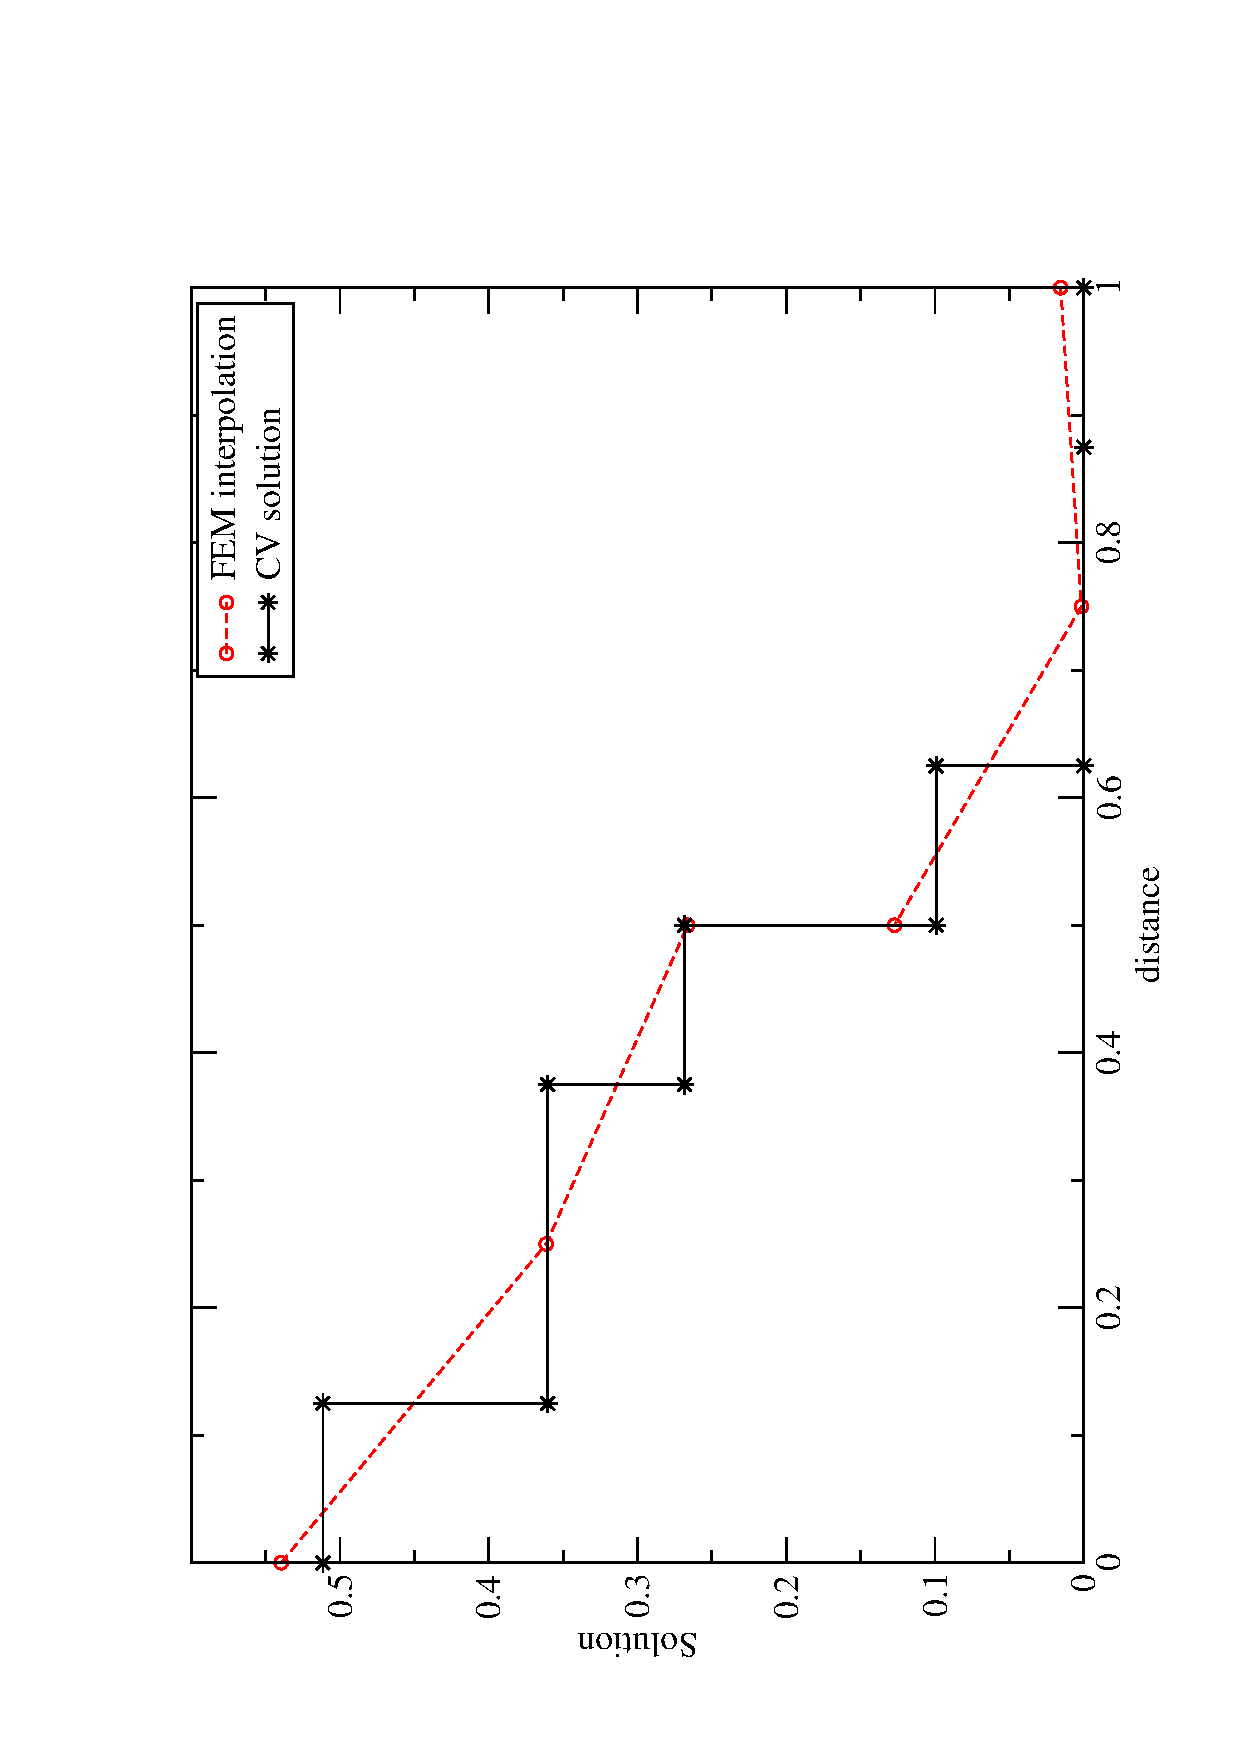
\includegraphics[width=1.\textwidth]{bl-dg-2eles}
\end{center}
\caption{Buckley-Leverett test-cases: Two element solution using the discontinuous formulation. Saturation field from both CV solution and FEM interpolation are shown.  \label{bl-dg-2eles}}
\end{figure}


%%%
%%%  FIGURE 
%%%
\begin{figure}[h]
\vbox{\hbox{\hspace{1.cm}
    \includegraphics[width=0.8\textwidth]{L1_convergence_rate_DG.eps}}
\vspace{.0cm}\hbox{\hspace{1.cm}
    \includegraphics[width=0.8\textwidth]{L2_convergence_rate_DG.eps}}}
    \caption{Buckley-Leverett test-cases: L1 (top) and L2 (bottom) error convergence rates for a number of fully discontinuous (between elements) element pairs. \label{fig:BL_converg-rates_DG}}
\end{figure}

%%%
%%%  FIGURE 
%%%
\begin{figure}[h]
\vbox{
\hbox{\hspace{.3cm}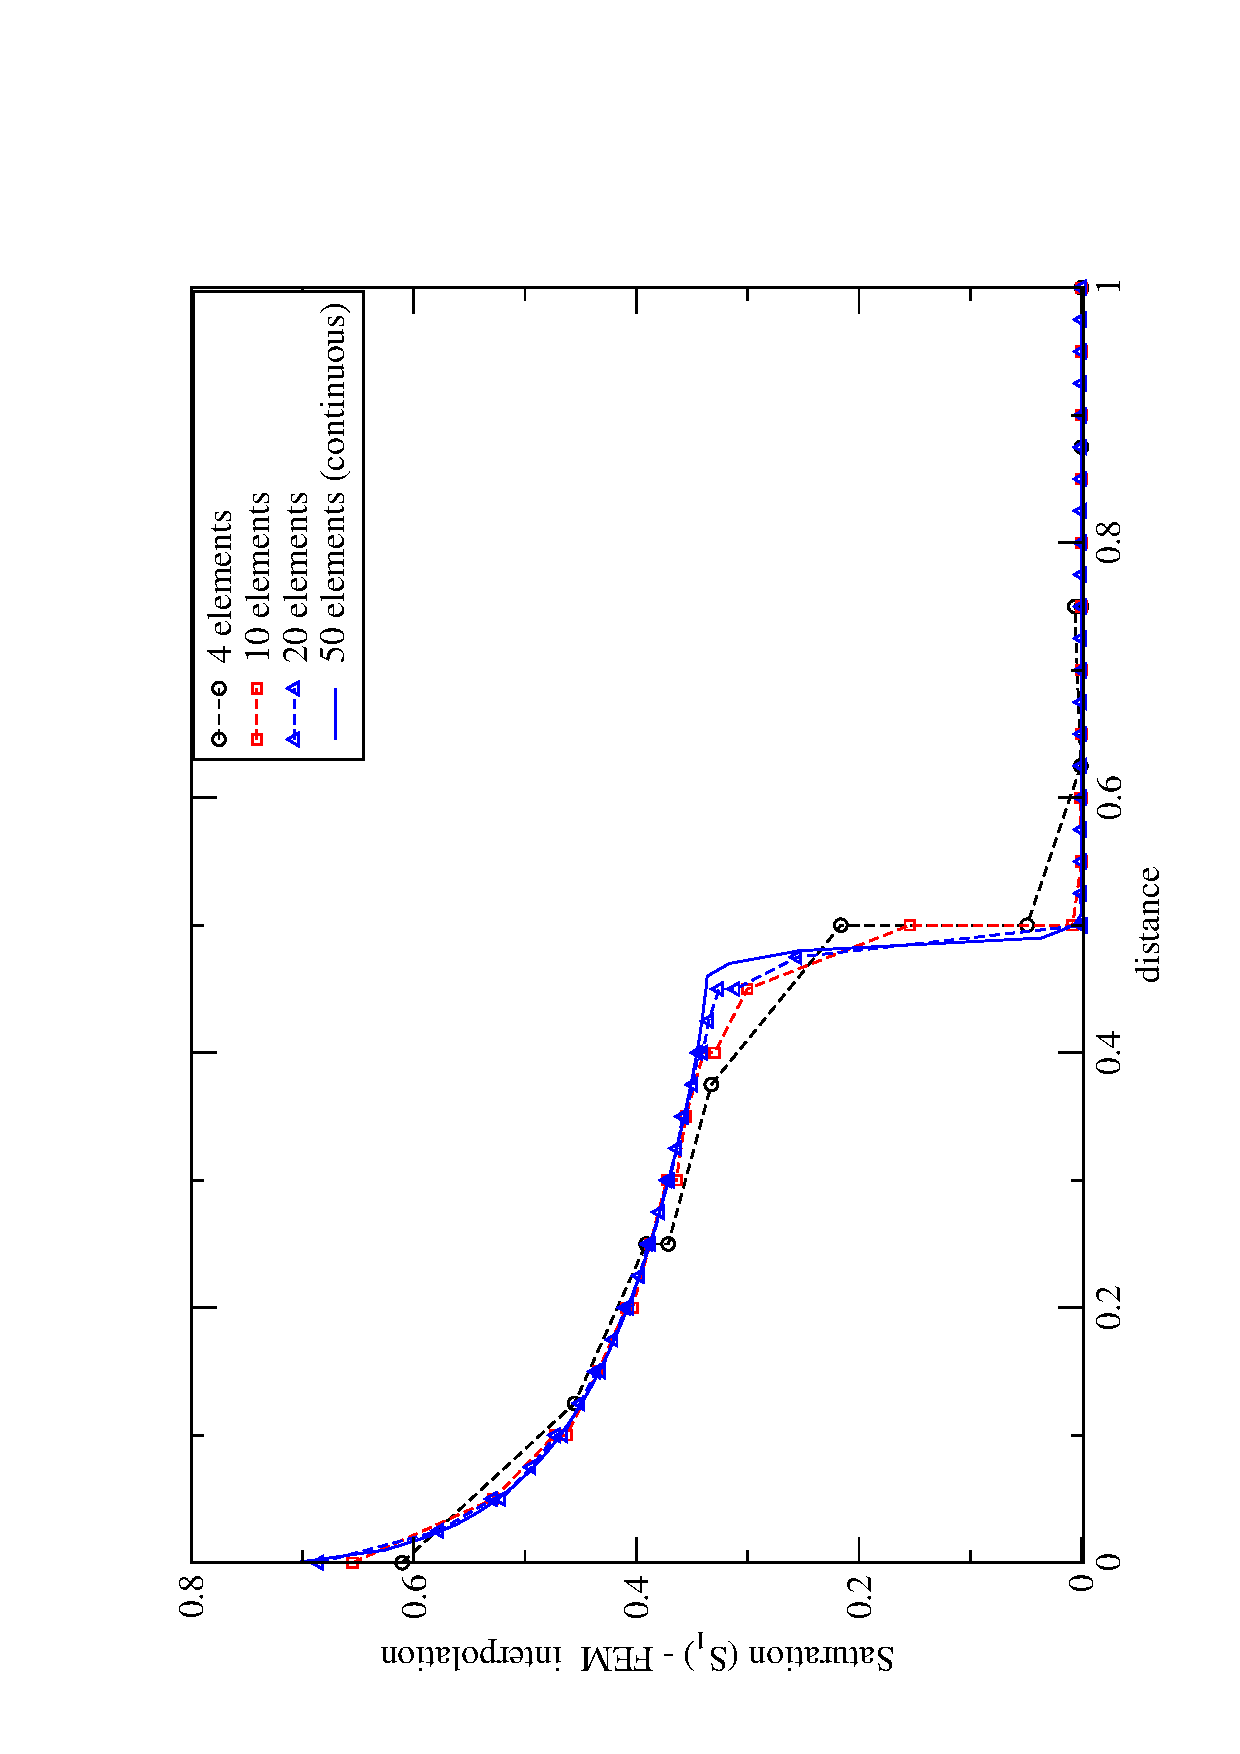
\includegraphics[width=.9\textwidth]{bl-dg-4-10-20}}
\vspace{-0.cm}
\hbox{\hspace{.3cm}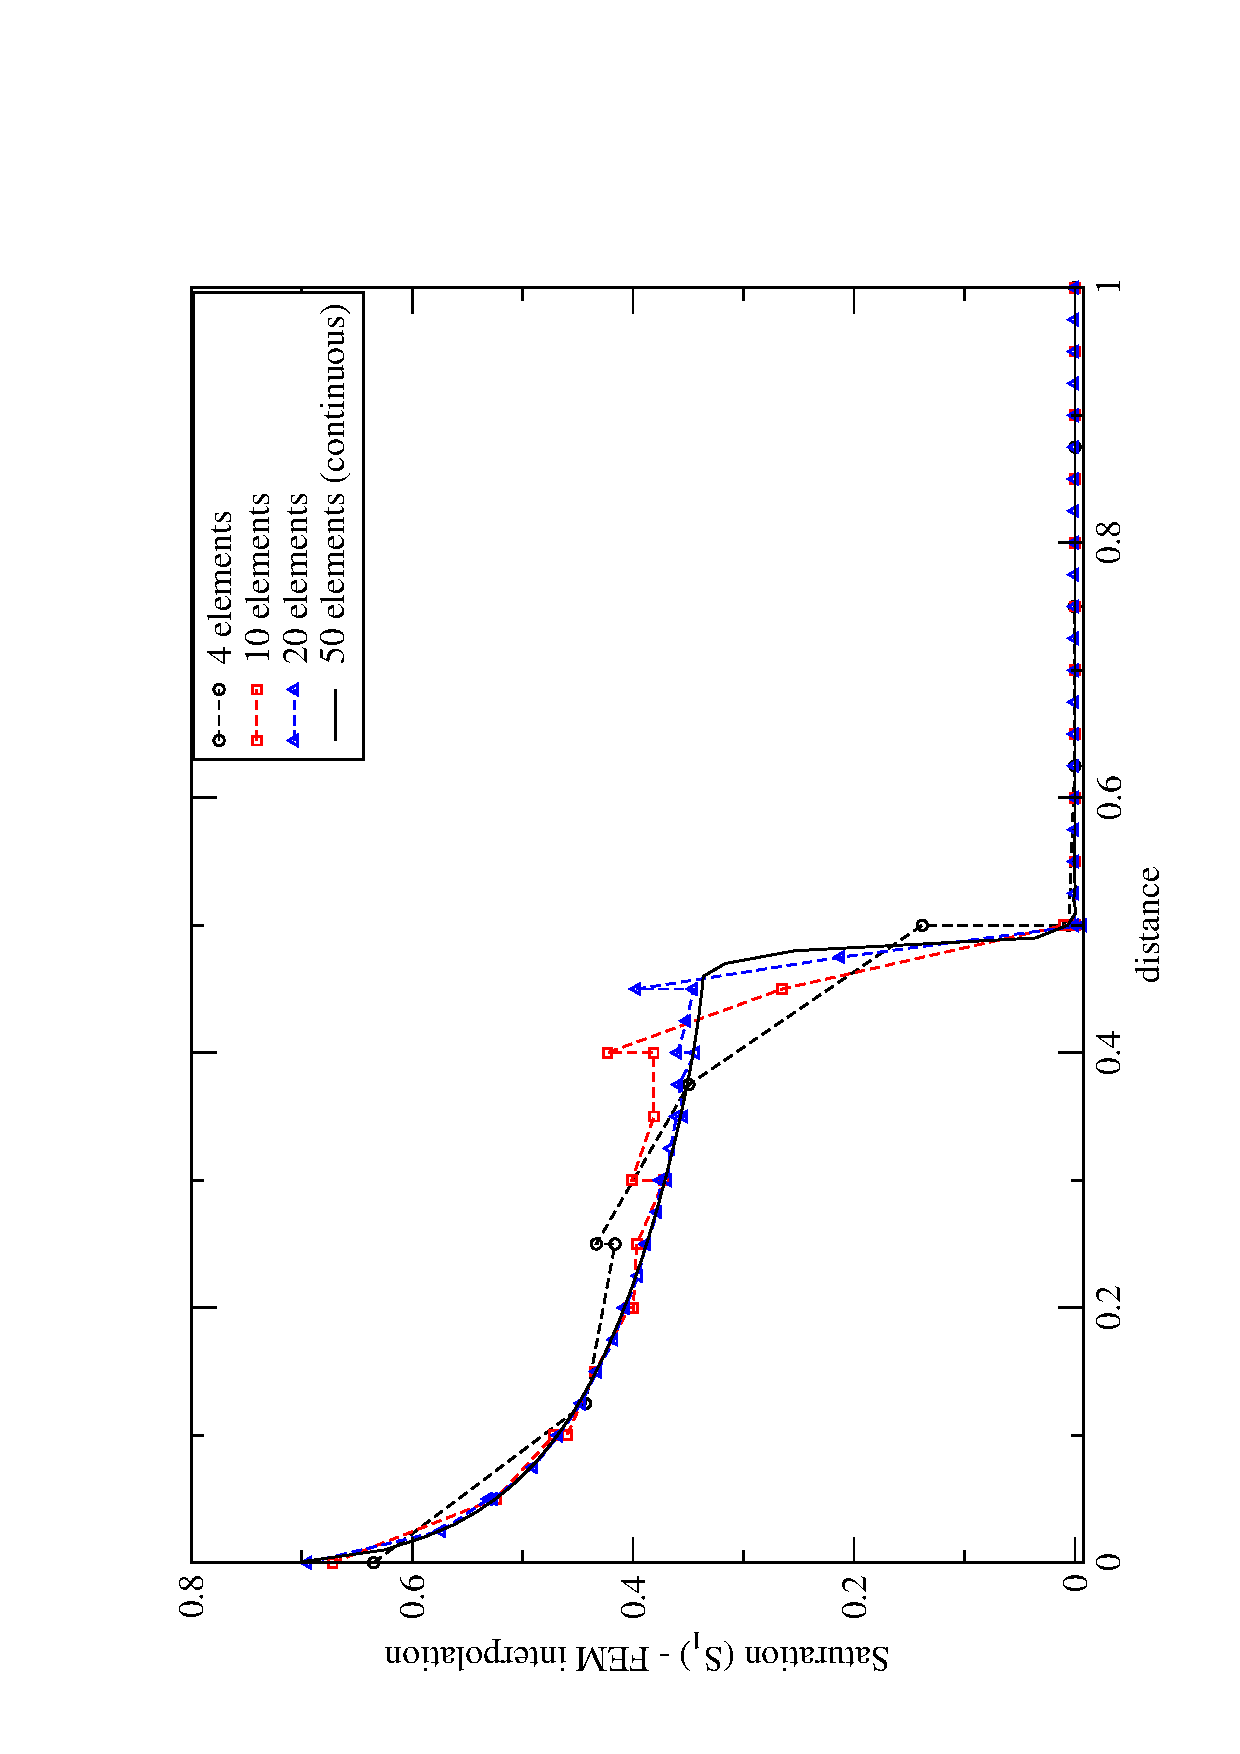
\includegraphics[width=.9\textwidth]{bl-dg-cent-4-10-20}}}
\caption{Buckley-Leverett test-cases: Saturation field obtained from the discontinuous and continuous formulation with different mesh resolutions. Solutions with (top) and without (bottom) upwinding scheme. Notice that oscillations are suppressed with the upwinding scheme.\label{bl-dg-cent-4-10-20}}
\end{figure}


%%%
%%%  FIGURE 
%%%
\begin{figure}[h]
\vbox{
\hbox{\hspace{.3cm}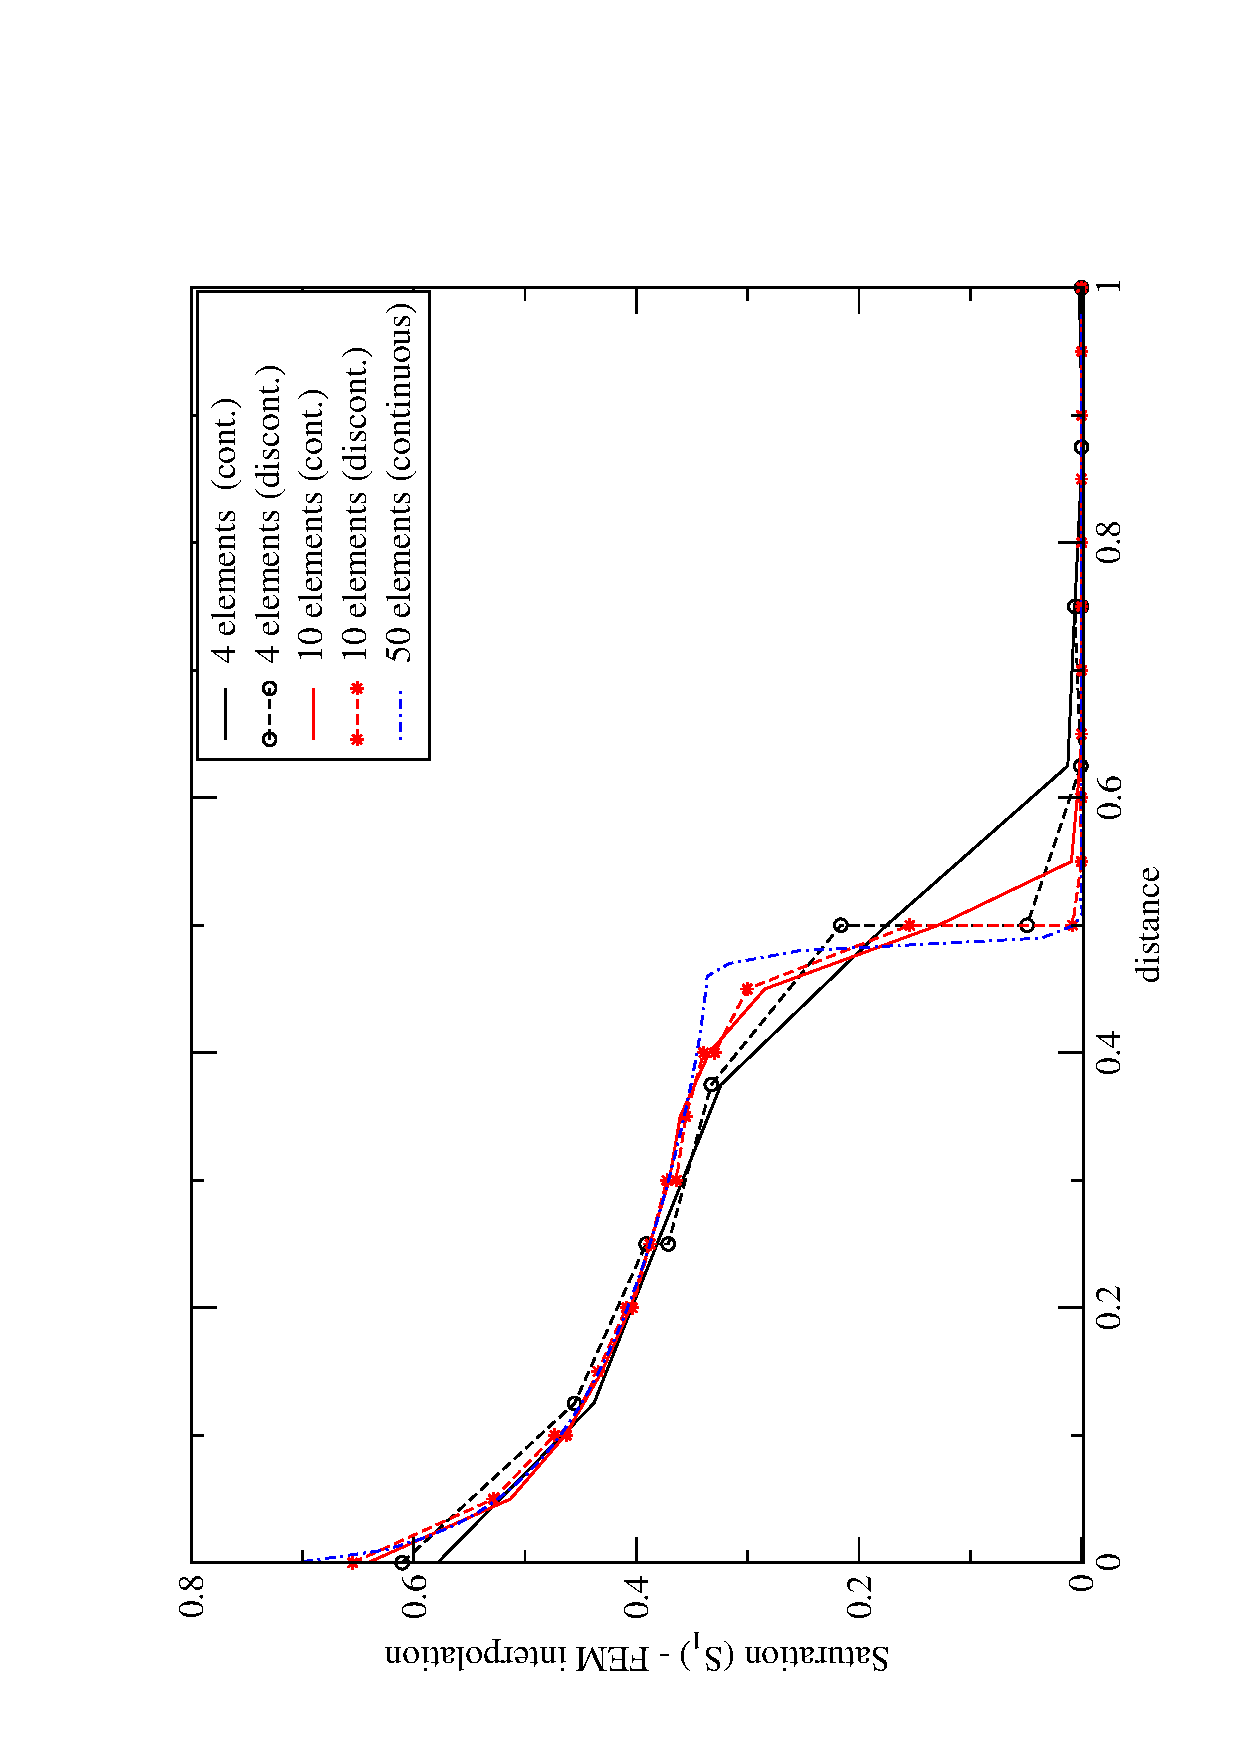
\includegraphics[width=.9\textwidth]{bl-dg-4-10-vers-cty}}
\vspace{-0.cm}
\hbox{\hspace{.3cm}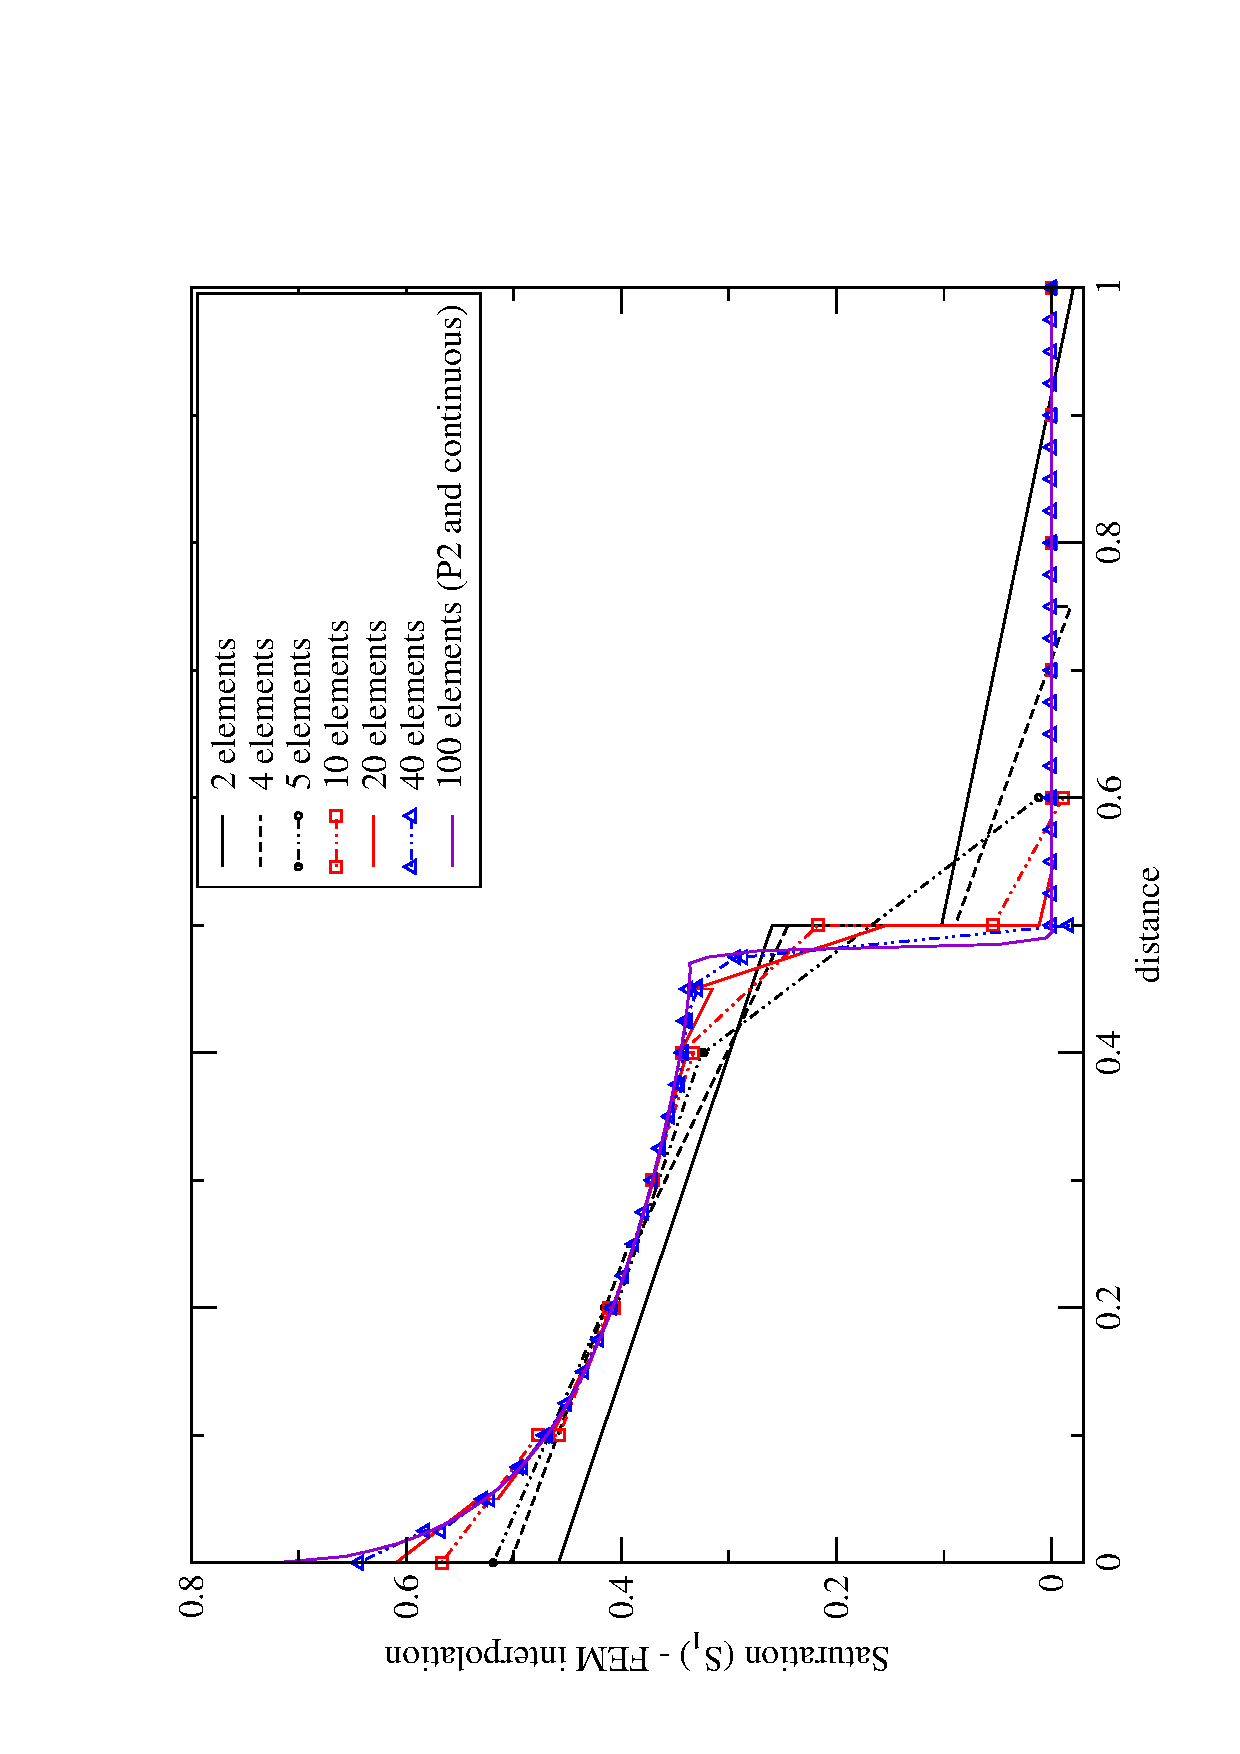
\includegraphics[width=.9\textwidth]{bl-dg-p1-2-4-5-10-20-40}}}
\caption{Buckley-Leverett test-cases: Saturation field obtained from (top) continuous and discontinuous (between elements) formulations (solution with 50 elements may be considered as a converged result). Solution obtained (bottom) from linear pressure (P1) formulation with different mesh resolution with comparison against P2-pressure formulation (continuous). \label{bl-dg-4-10-vers-cty}}
\end{figure}


%%%
%%%  FIGURE 
%%%
\begin{figure}[h]
\vbox{
\hbox{\hspace{.2cm}
    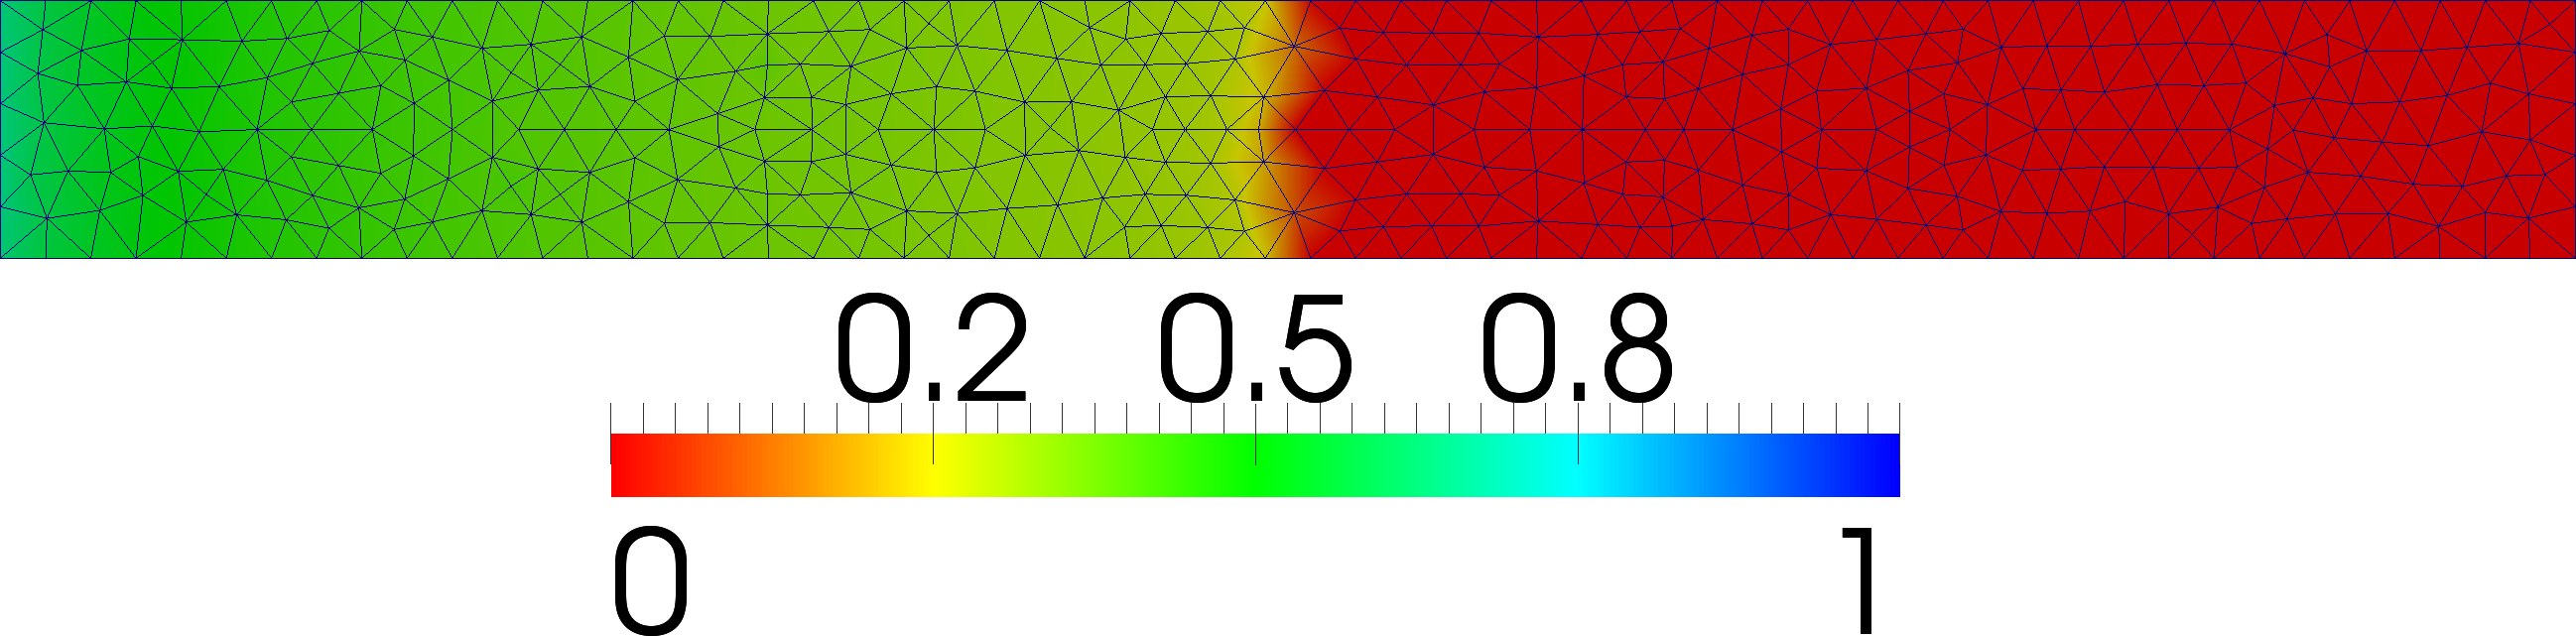
\includegraphics[width=1.\textwidth]{map_2d.png}}
\vspace{1.cm}
\hbox{\hspace{0.2cm}
    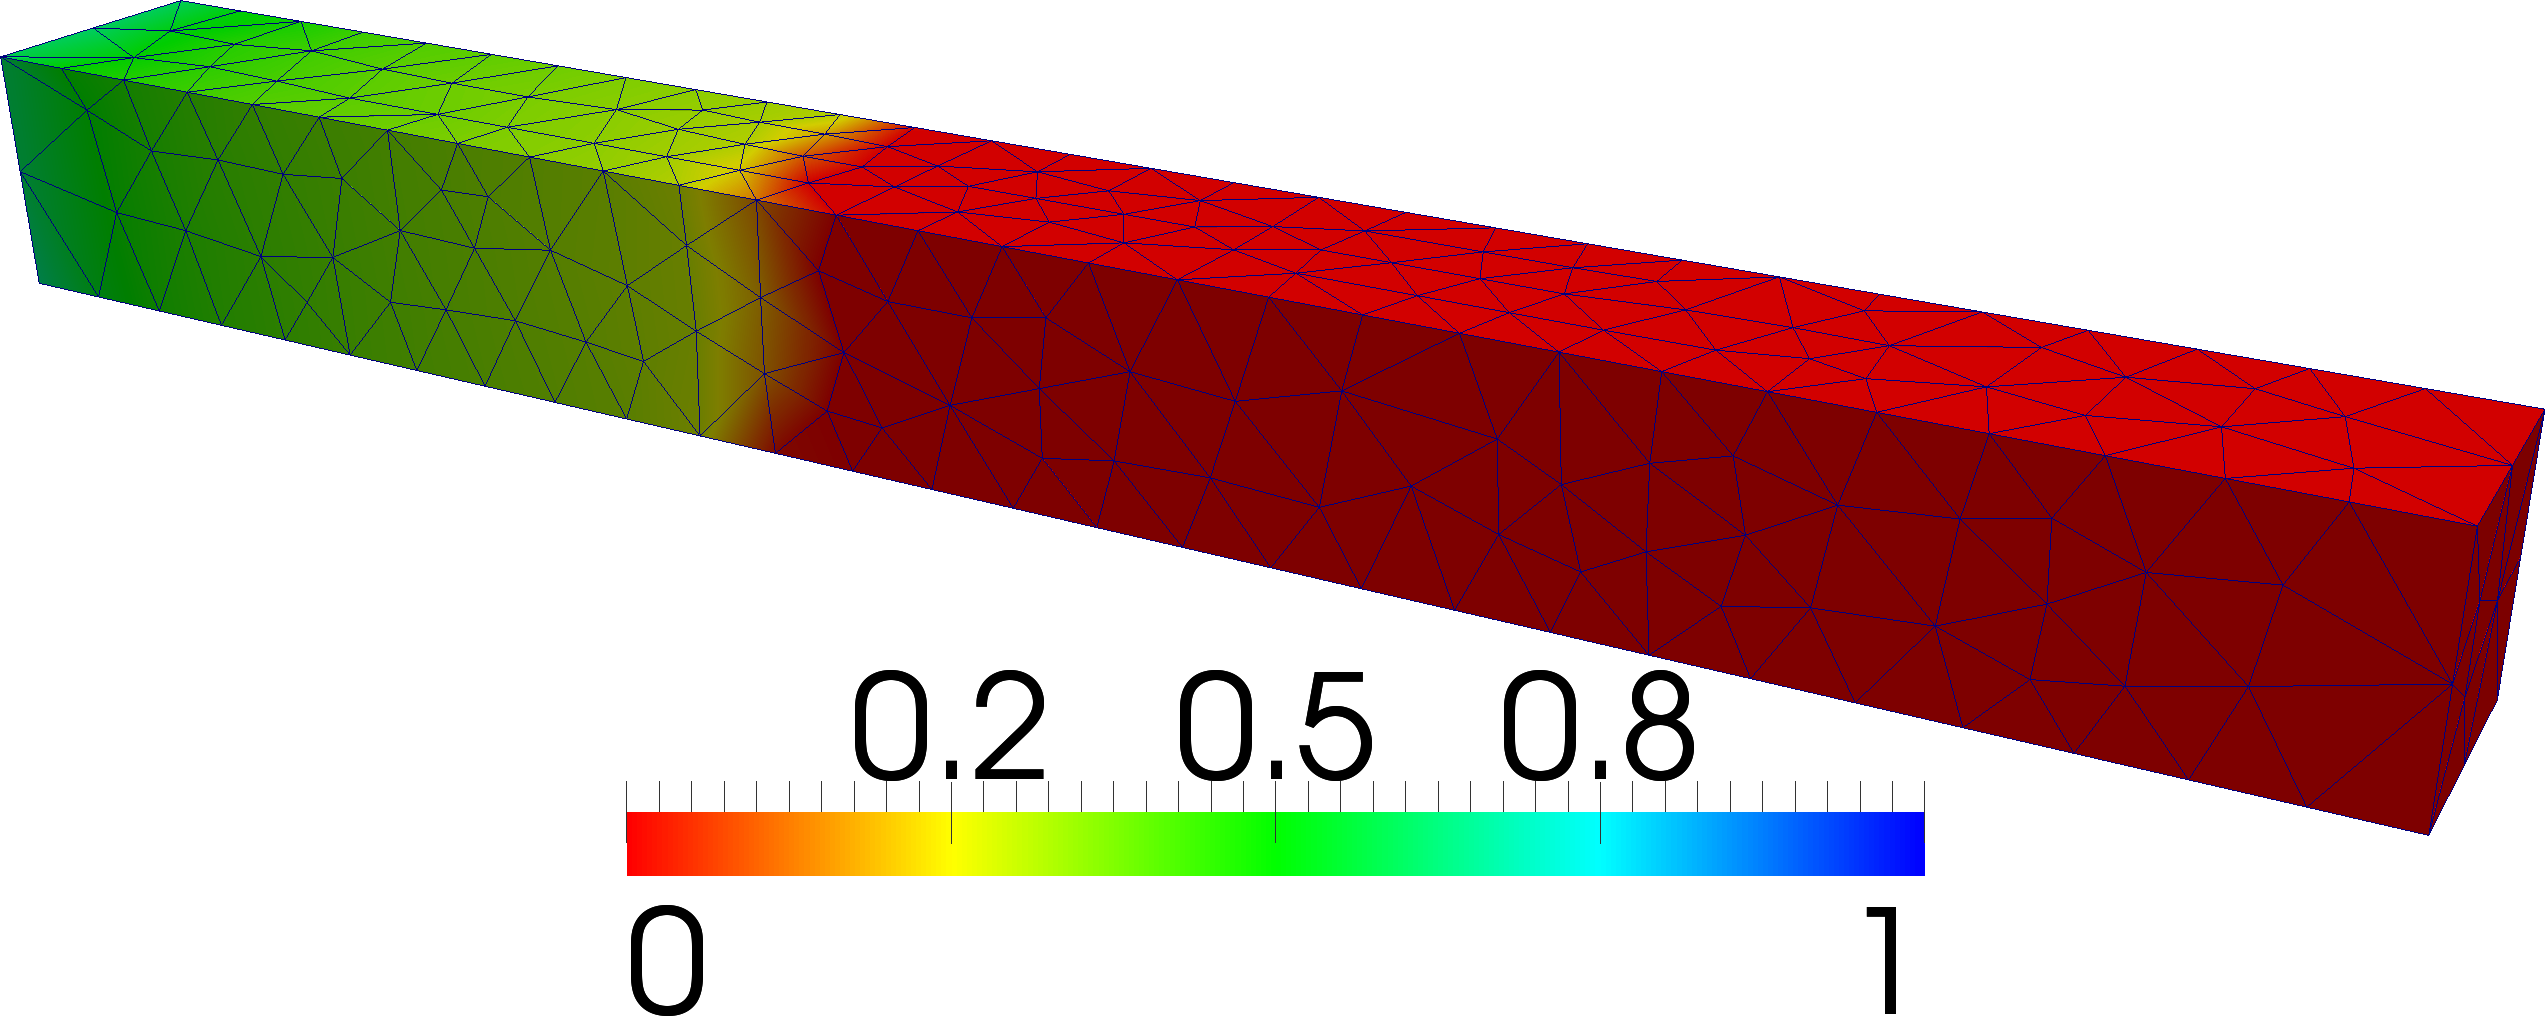
\includegraphics[width=1.\textwidth]{map_3d.png}}}
    \caption{Buckley-Leverett test-cases: phase 1 saturation surface maps for a 2- (770 triangles) and 3-D (1207 tetrahedra) simulations (\PN[1]{2} unstructured mesh grids) at time $t=0.5$. \label{fig:maps2d_3d}}
\end{figure}


%%%  FIGURE 
%%%
\begin{figure}[h]
\vbox{\hbox{\hspace{.3cm}
    \includegraphics[width=0.9\textwidth]{BL_2d_P1DGP2_convergence.eps}}
\vspace{-.0cm}\hbox{\hspace{.3cm}
    \includegraphics[width=0.9\textwidth]{simulations_2d_3d.eps}}}
    \caption{Buckley-Leverett test-cases: 2- and 3-D phase 1 saturation profiles with \PN[1]{2} elements. Sensitivity analysis for (top) grid resolution using structured \PN[1]{2} mesh, and (bottom) mesh type.\label{fig:BL_2d_profiles}}
\end{figure}



%%%
%%%  FIGURE 
%%%
\begin{figure}[h]
  \begin{center}
    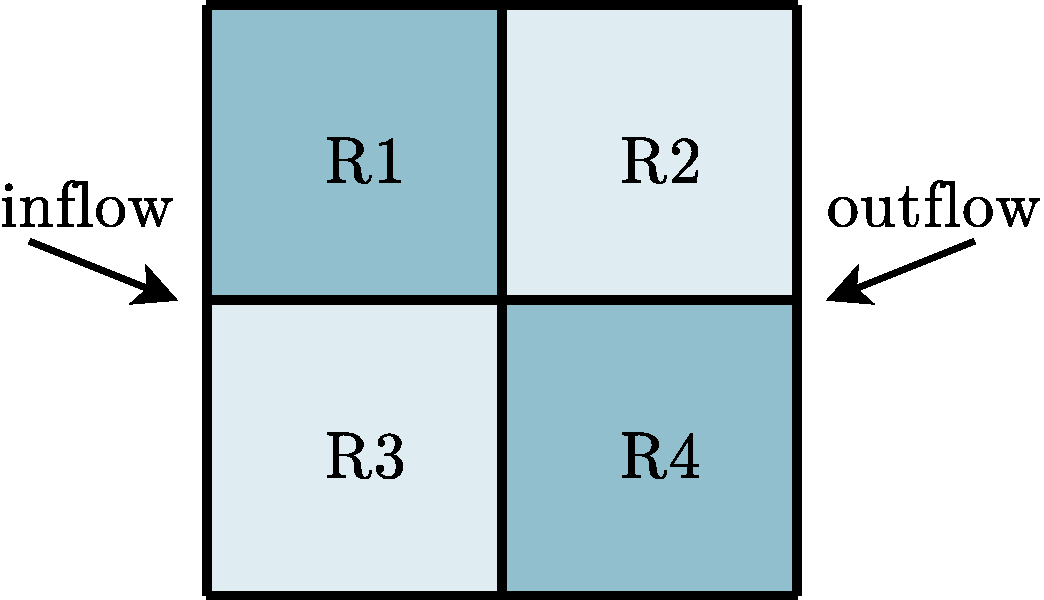
\includegraphics[width=0.65\textwidth]{4Rregion_BL}
    \caption{Heterogeneous permeability test-cases: schematic including boundary conditions. Darker areas (R1 and R4) represent regions with high permeability.\label{fig:4reg_BL_schematic}}
  \end{center}
\end{figure}

%%%
%%%  FIGURE 
%%%
\begin{figure}[h]
\vbox{\hbox{
\hspace{-1.8cm}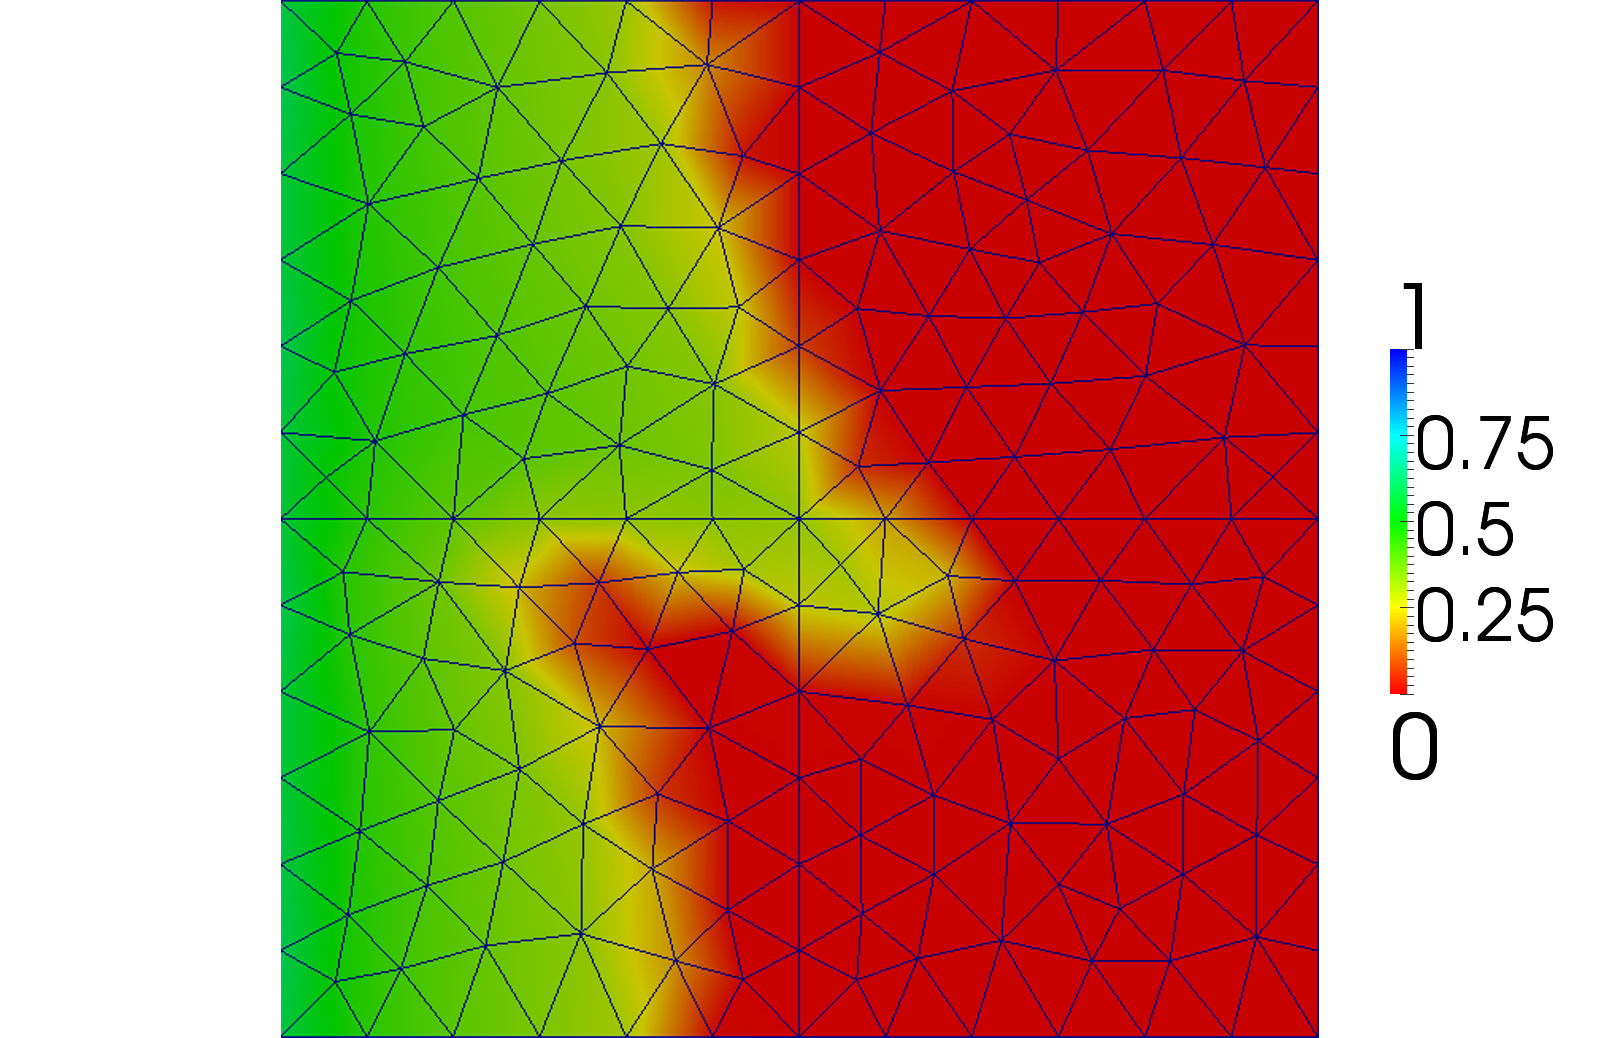
\includegraphics[width=0.6\textwidth]{CG_coarse083.png}
\hspace{-0.2cm}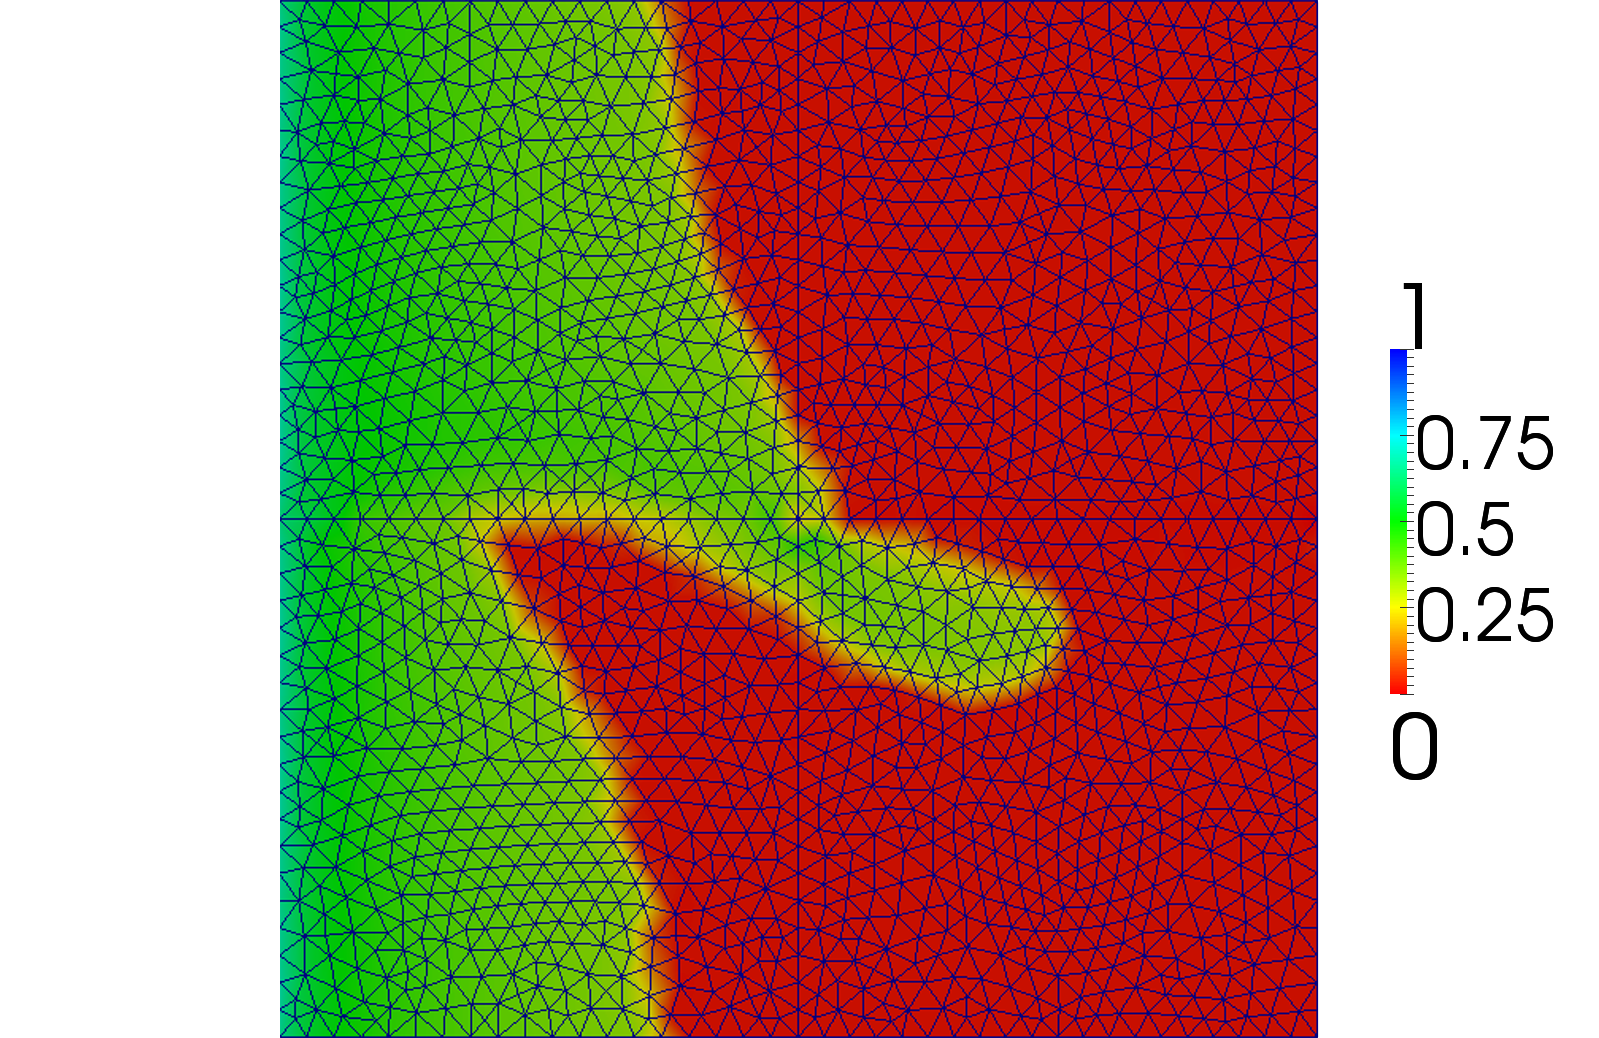
\includegraphics[width=0.6\textwidth]{CG_fine083.png}}
\vspace{1.cm}\hbox{
\hspace{-1.8cm}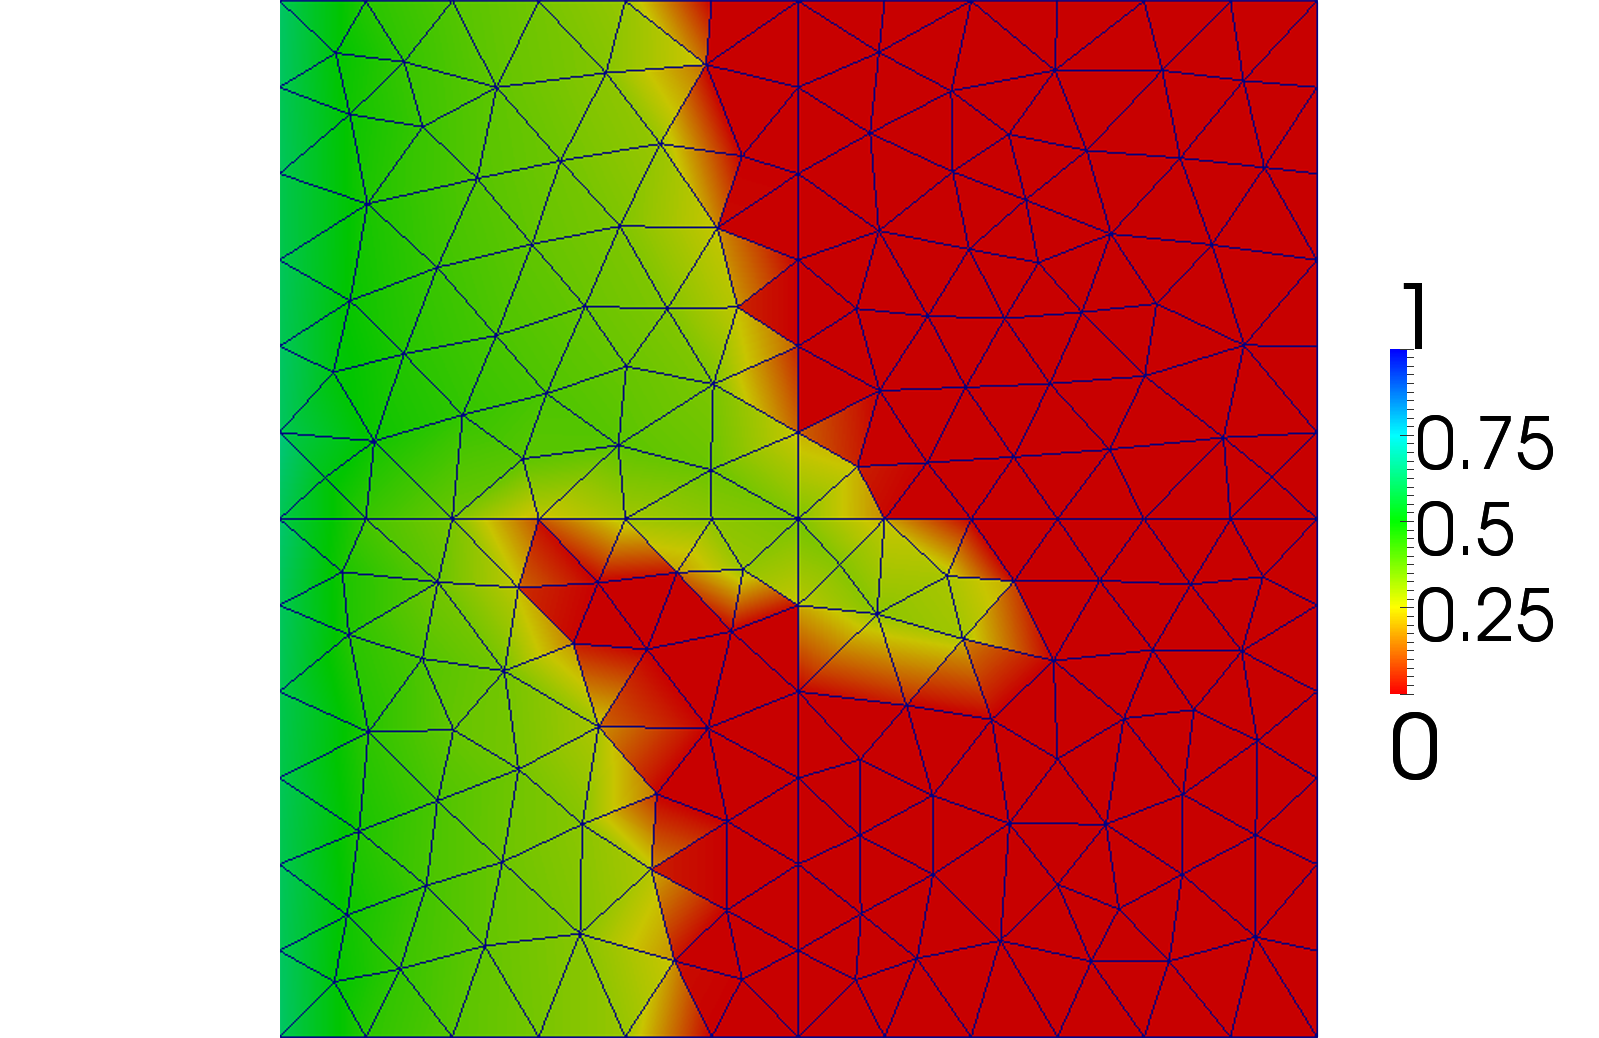
\includegraphics[width=0.6\textwidth]{DG_coarse083.png}
\hspace{-0.2cm}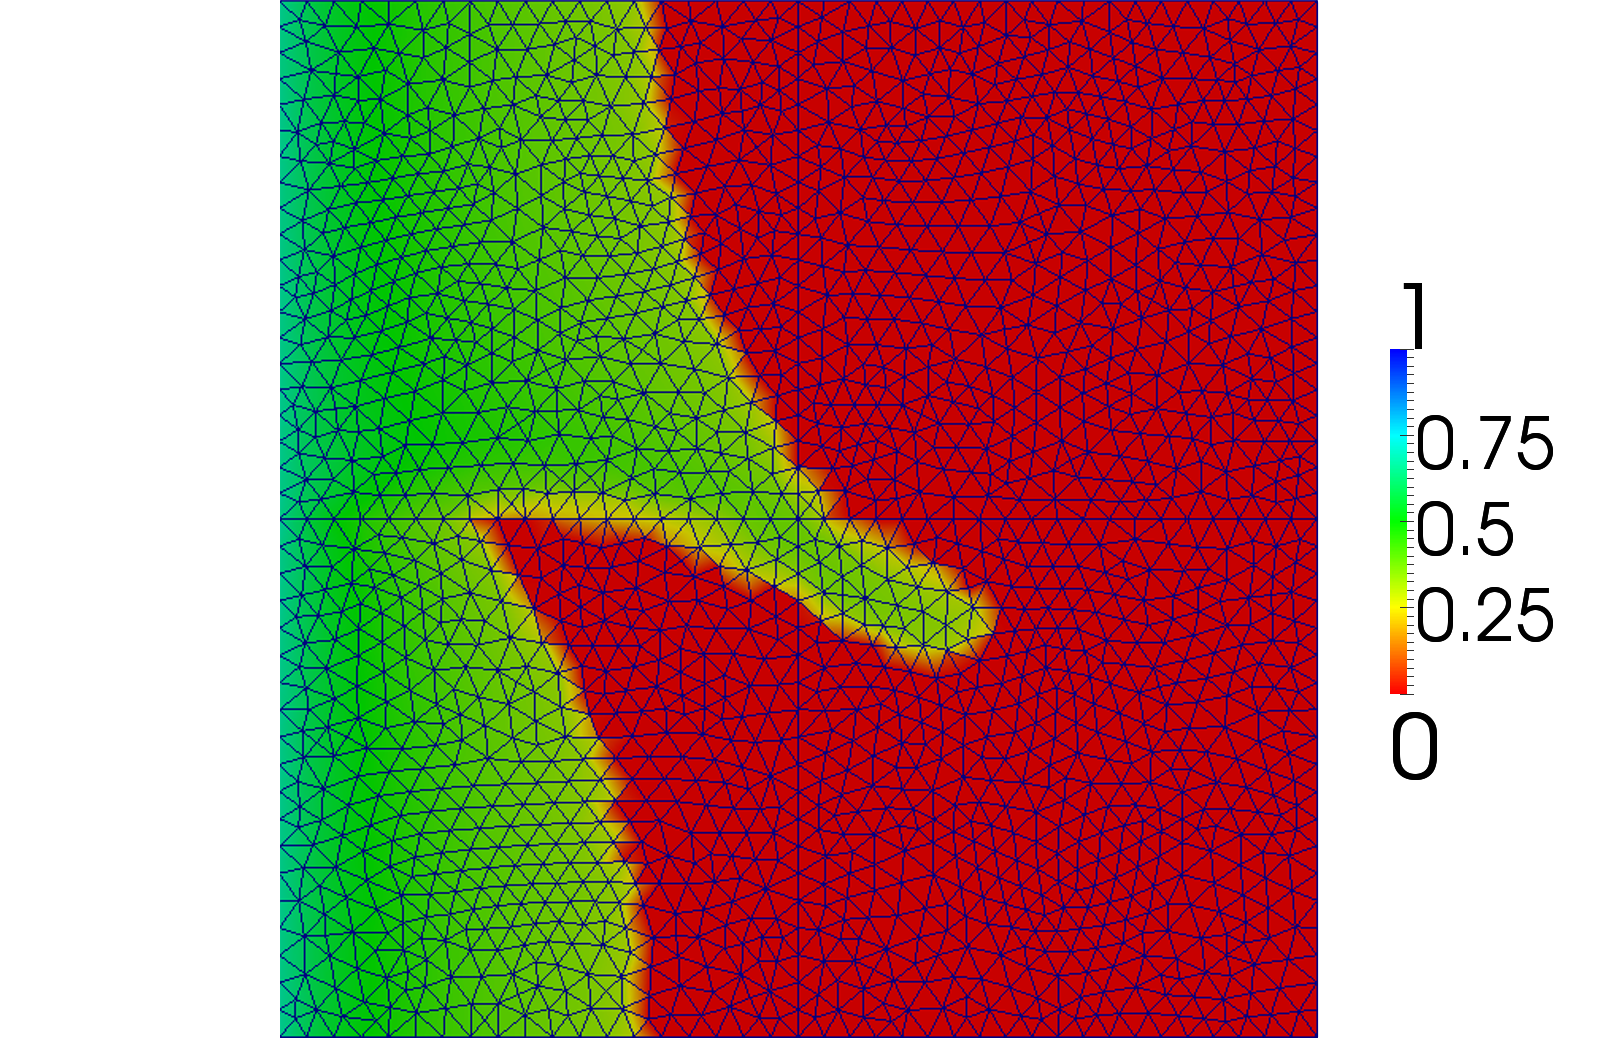
\includegraphics[width=0.6\textwidth]{DG_fine083.png}}}
 \caption{Heterogeneous permeability test-cases: phase 1 saturation maps at time $t=0.08$ seconds. Upper- and lower-rows show saturation fronts (superimposed with unstructured mesh) calculated with \PN[1]{2} and \PN[2]{2}DG elements, respectively. Left/Right columns: 402 triangles (2412 nodes) and 3714 triangles (22284 nodes) meshes.\label{fig:4reg_maps}}
\end{figure}

%%%
%%%  FIGURE 
%%%
\begin{figure}[h]
  \begin{center}
    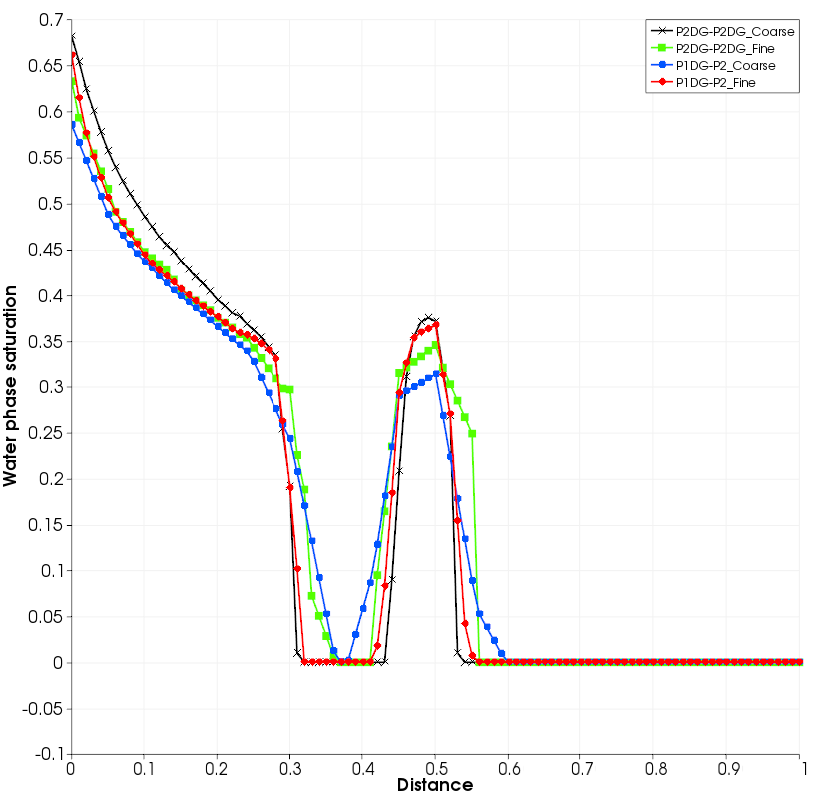
\includegraphics[width=0.475\textwidth]{down_left_top_right083}
    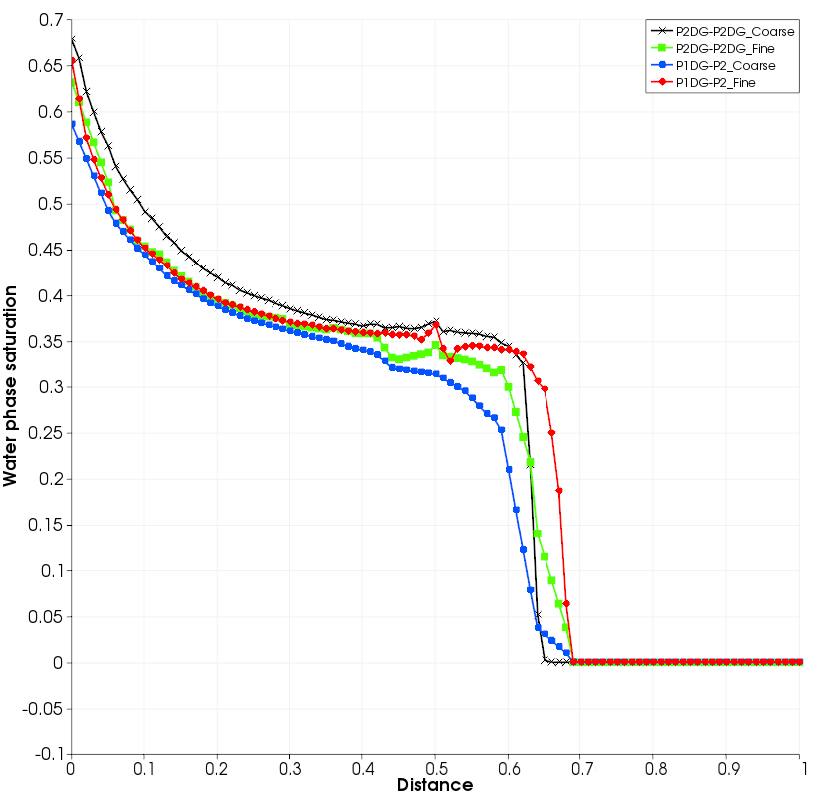
\includegraphics[width=0.475\textwidth]{Top_left-Down_right083}
    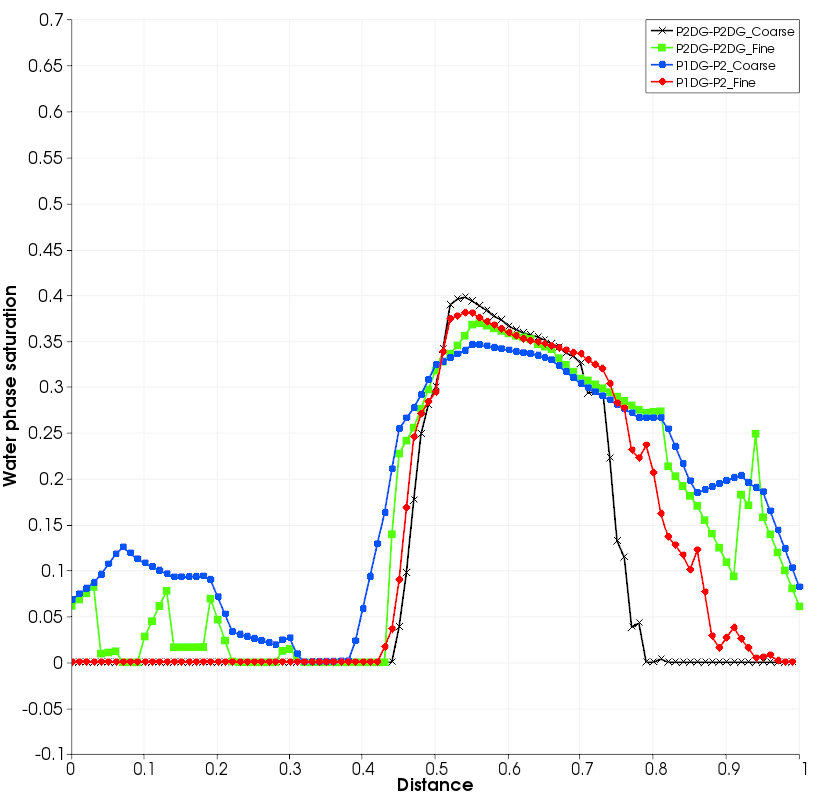
\includegraphics[width=0.475\textwidth]{X04_083}
    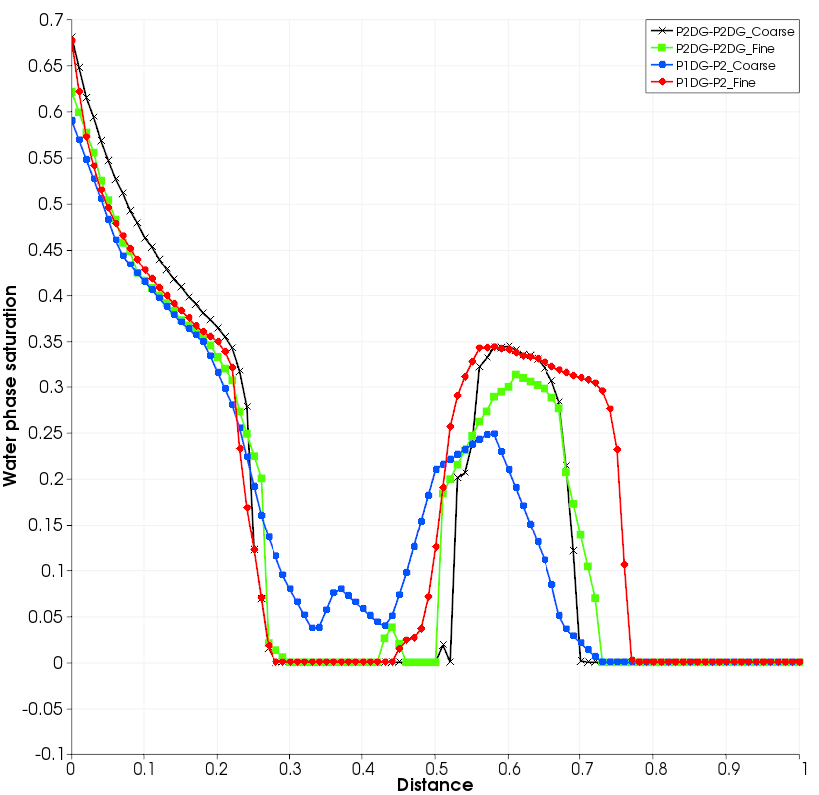
\includegraphics[width=0.475\textwidth]{y04_083}
    \caption{Heterogeneous permeability test-cases: phase 1 saturation profiles at time $t=0.08$ seconds. Top left: profiles at the diagonal starting at the bottom left corner of the domain. Top right: profiles at the diagonal starting at the top left corner of the domain. Bottom left: profiles at $x=0.4$. Bottom right: profiles at $y=0.4$.\label{fig:4reg_plots}}
  \end{center}
\end{figure}



%%%
%%%  FIGURE 
%%%
\begin{figure}[h]
\vbox{
\hbox{
\hspace{3.5cm} 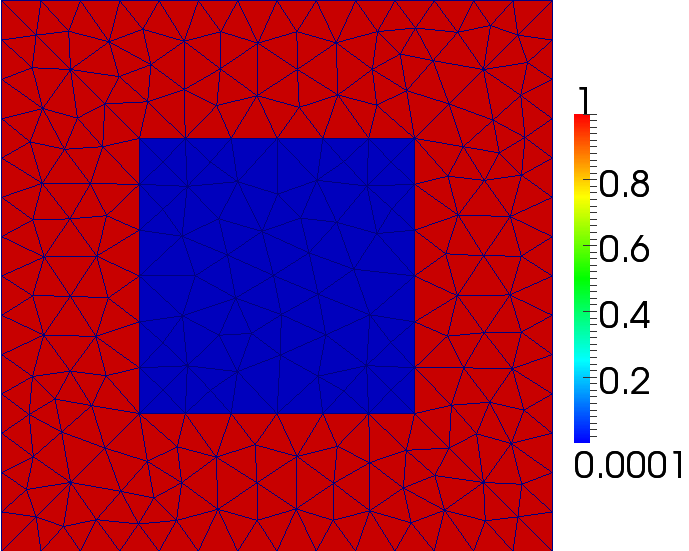
\includegraphics[width=0.5\textwidth]{square_permeability_low}}
\vspace{0.5cm}
\hbox{
\hspace{-0.cm}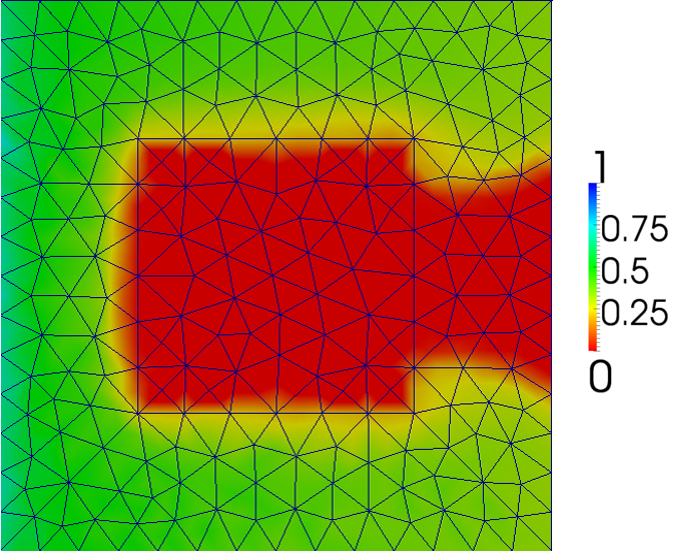
\includegraphics[width=0.5\textwidth]{cg_square_015_low}
\hspace{-0.cm}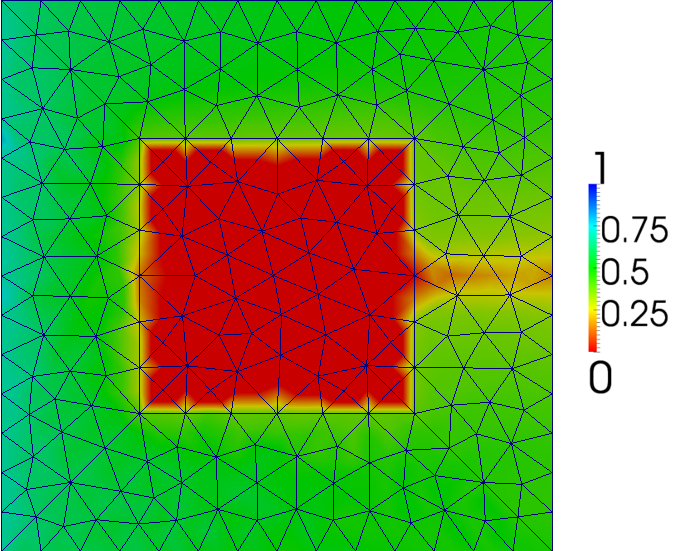
\includegraphics[width=0.5\textwidth]{cg_square_05_low}}
\vspace{0.5cm}
\hbox{
\hspace{-0.cm}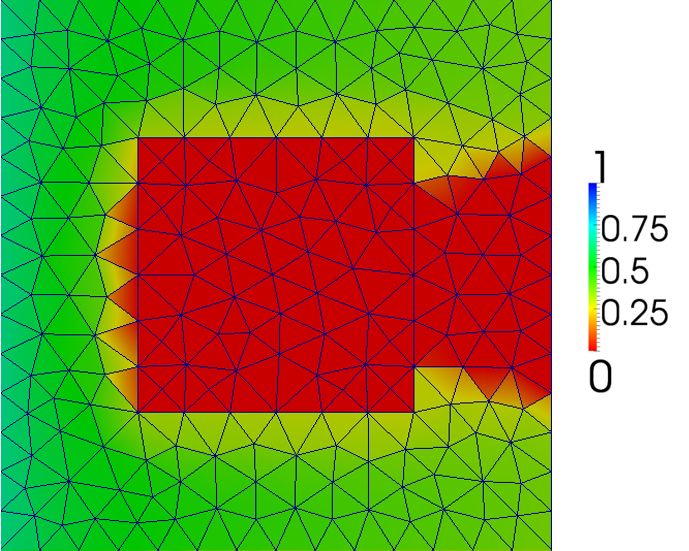
\includegraphics[width=0.5\textwidth]{dg_square_015_low}
\hspace{-0.cm}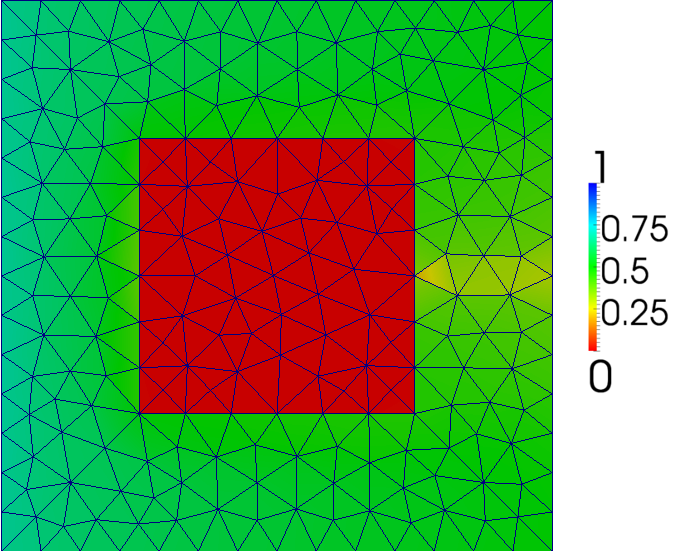
\includegraphics[width=0.5\textwidth]{dg_square_05_low}}}
 \caption{Underground Caisson: Initial configuration of porous matrix consisting of a low-permeability square embedded in a high-permeability region (top). Phase 1 saturation profile at 0.15 (left) and 0.5 seconds (right) within the transient for simulation performed using \PN[0]{1} (middle) and \PN[1]{1}DG (bottom) element-pairs.\label{fig:square_permeability}}
\end{figure}

%%%
%%%  FIGURE 
%%%

\begin{figure}[h]
\vbox{
\hbox{
\hspace{-0.cm}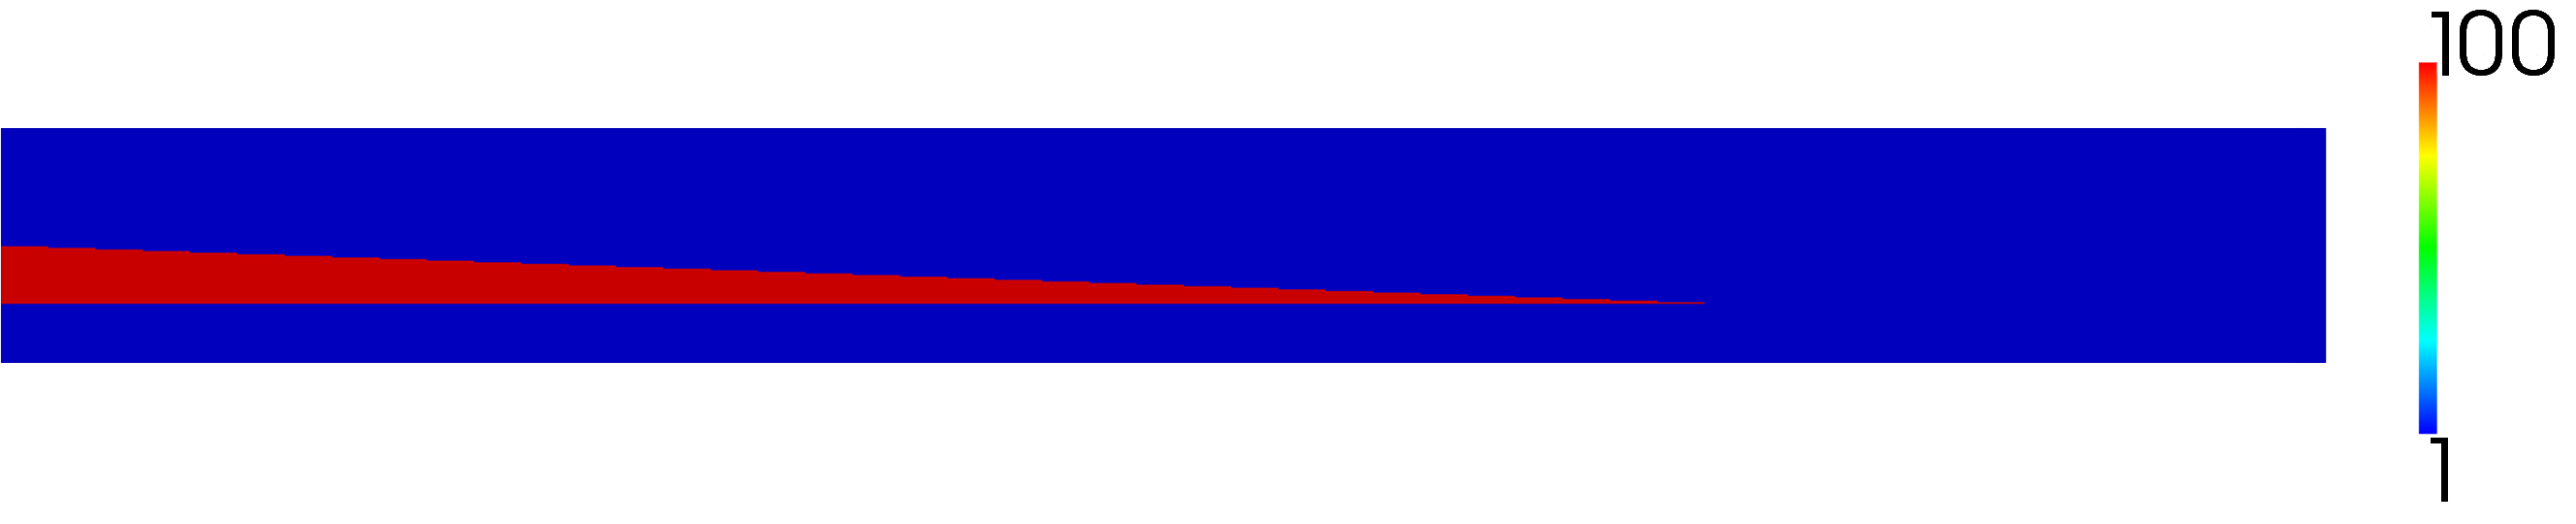
\includegraphics[width=1.05\textwidth]{wedge_permeability}}
\vspace{-1.cm}\hbox{\hspace{4cm}(a) Permeability map}
\vspace{.5cm}
\hbox{
\hspace{-0.cm}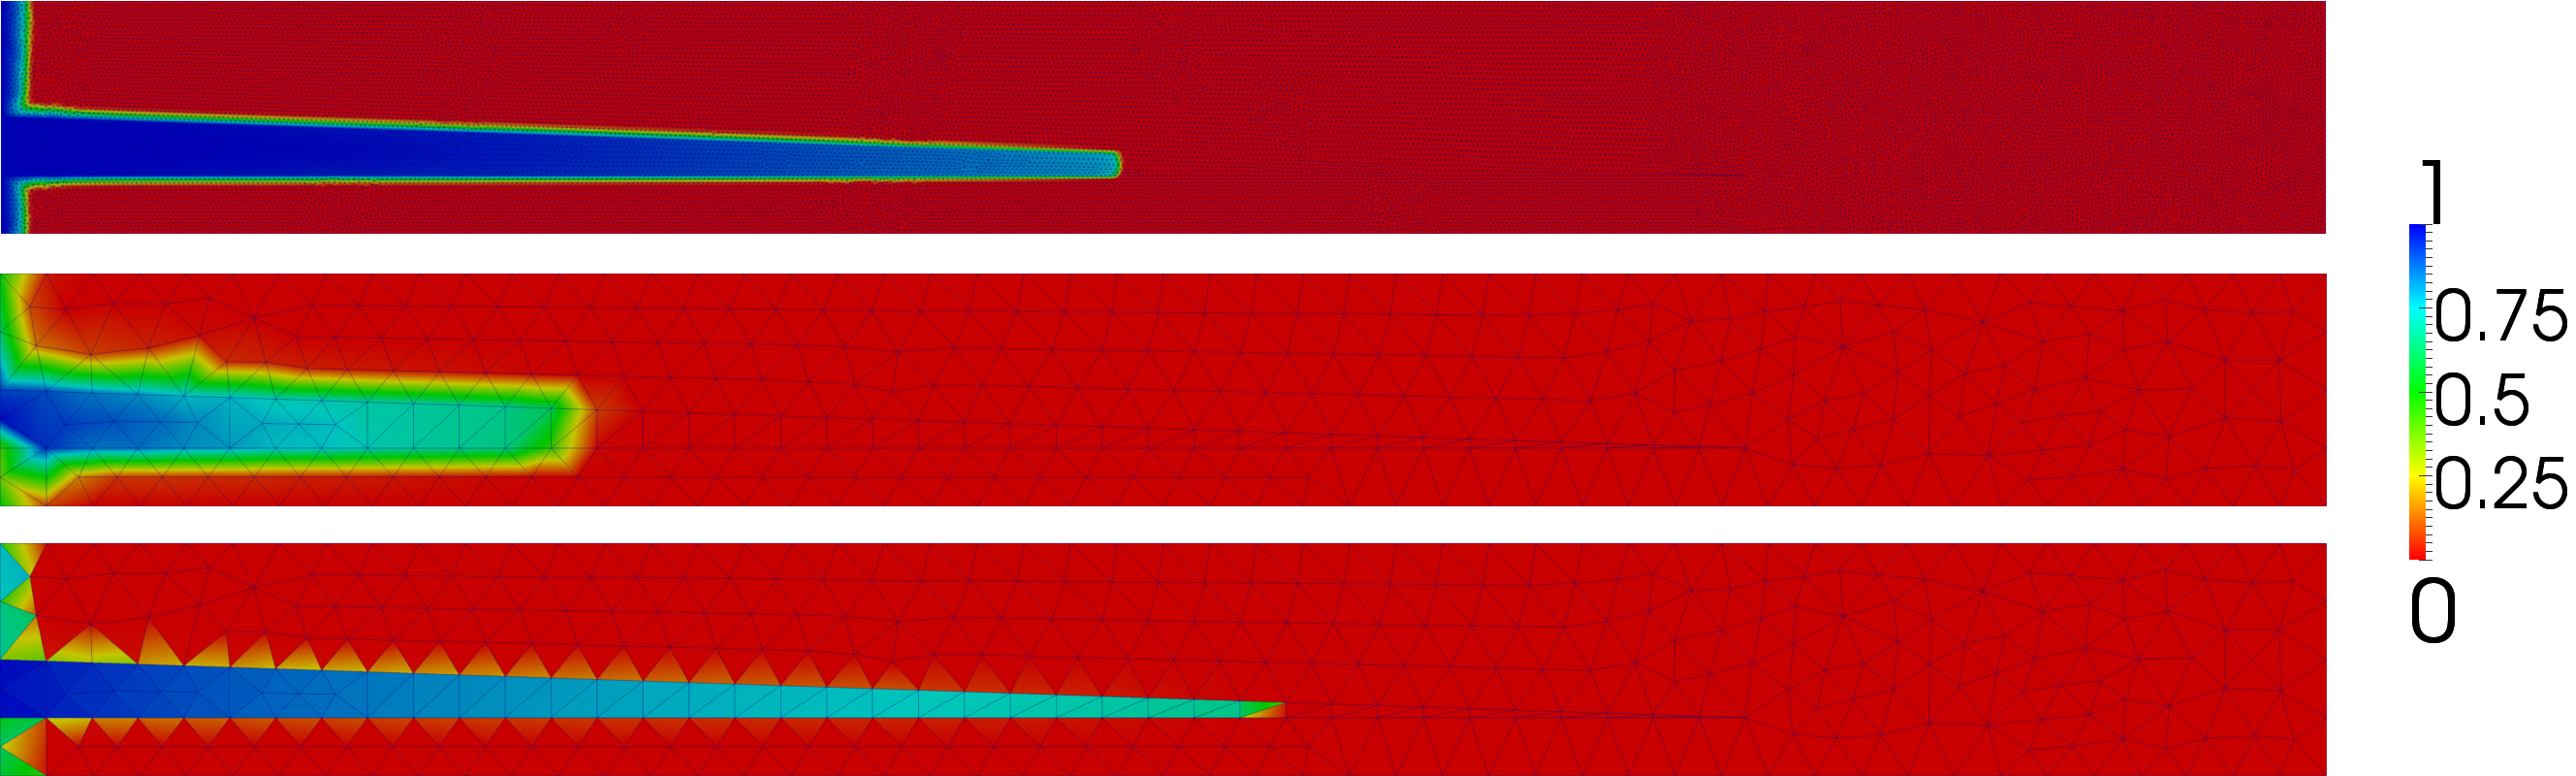
\includegraphics[width=1.05\textwidth]{wedge_0011}}
\vspace{-0.cm}\hbox{\hspace{4cm}(b) $t= 0.011$ seconds }
\vspace{.5cm}
\hbox{
\hspace{-.cm}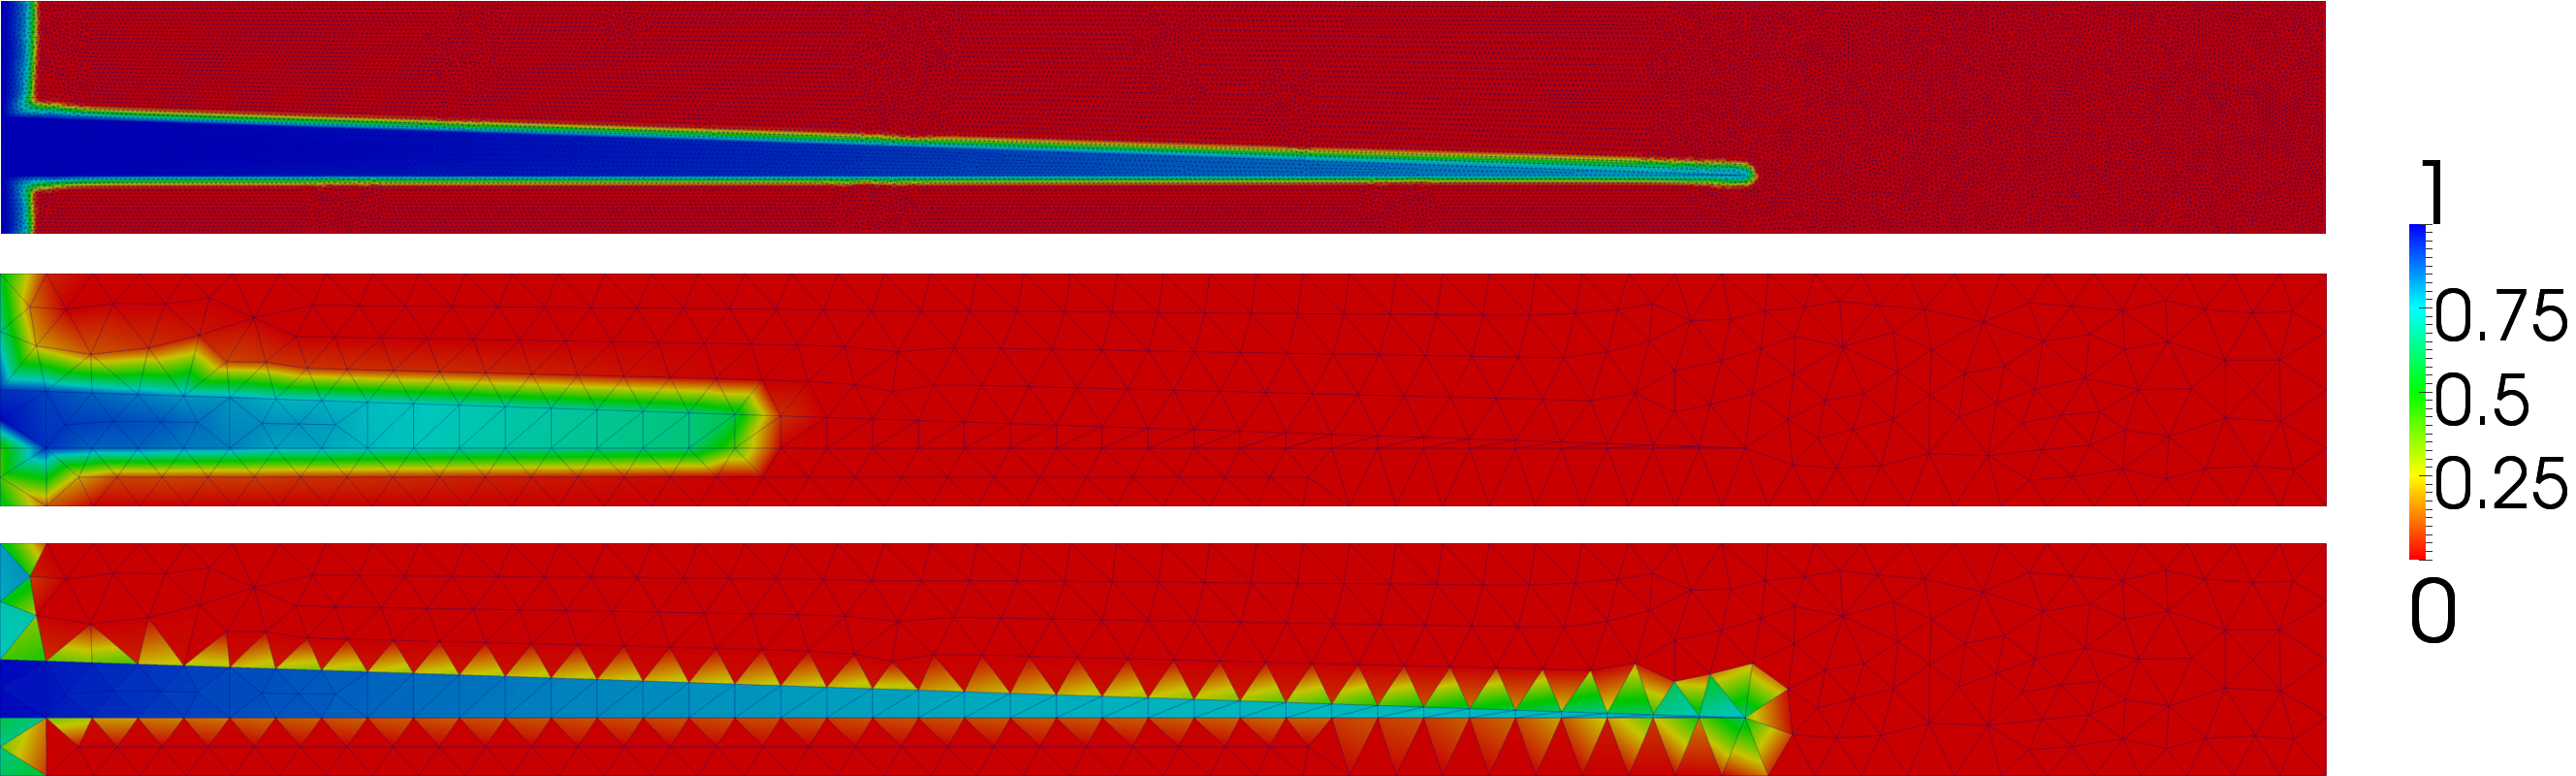
\includegraphics[width=1.05\textwidth]{wedge_0014}}
\vspace{-0.cm}\hbox{\hspace{4cm}(b) $t= 0.014$ seconds }
}
\caption{Wedged-shaped region: (a) two phase flow in a rectangular domain with an internal wedge-shaped region with high-permeability. Snapshots of water-phase saturation profiles of simulations performed with a fine mesh \PN[0]{1} simulation (top) 
and course mesh \PN[0]{1} simulation (middle)  and course mesh \PN[2]{1}DG simulation (bottom) at (b) 0.011 and (c) 0.0014 seconds.\label{fig:wedge_permeability}}
\end{figure}


%%%
%%%  FIGURE 
%%%

\begin{figure}[h]
\vbox{
\hbox{
\hspace{-0.cm}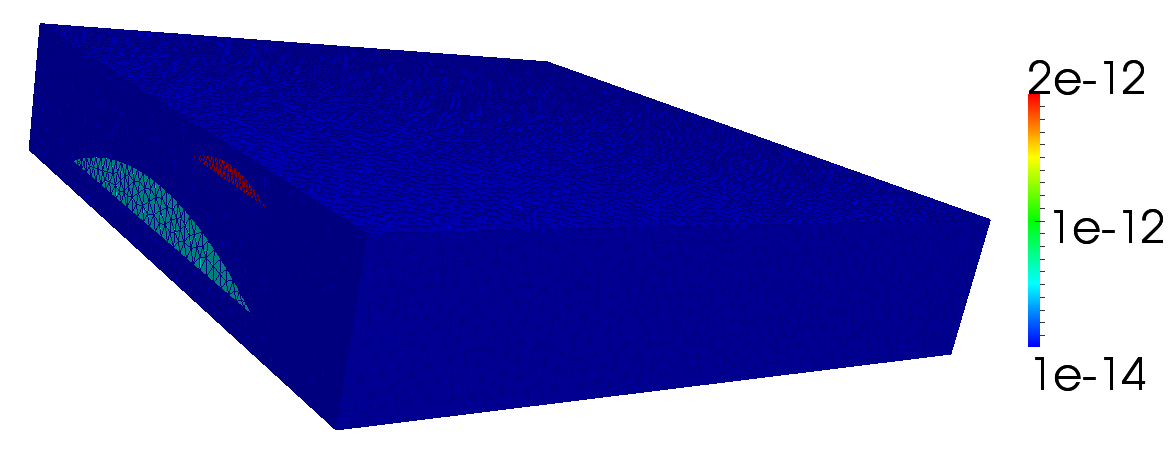
\includegraphics[width=0.85\textwidth]{3d_perm}}
\vspace{-0.cm}\hbox{\hspace{4cm}(a) Permeability map}
\vspace{.5cm}
\hbox{
\hspace{-0.cm}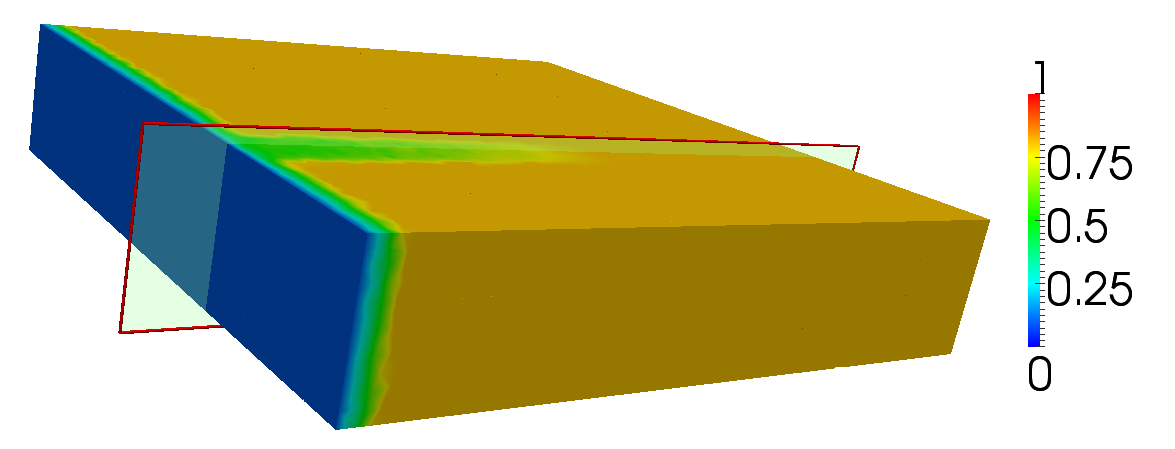
\includegraphics[width=0.85\textwidth]{3d_first}}
\vspace{-0.cm}\hbox{\hspace{4cm}(b) $t= 7.9$ years }
\vspace{.5cm}
\hbox{
\hspace{-.cm}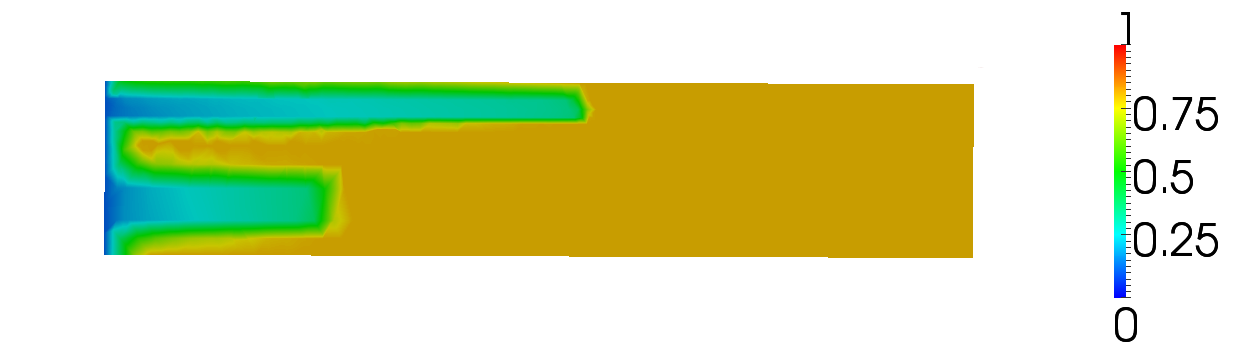
\includegraphics[width=0.85\textwidth]{3d_second}}
\vspace{-0.cm}\hbox{\hspace{4cm}(c) Internal section }
}
\caption{Hexahedron domain: (a) Permeability map and mesh used. Snapshots of water-phase saturation profiles of simulations performed with \PN[0]{1} (b) 3-D solution and (c) 2-D internal slice.\label{fig:3d_perm}}
\end{figure}

